% Options for packages loaded elsewhere
\PassOptionsToPackage{unicode}{hyperref}
\PassOptionsToPackage{hyphens}{url}
%
\documentclass[
]{book}
\title{Miller Creek and Vogel Lake Water Quality}
\author{Benjamin Meyer (\href{mailto:ben@kenaiwatershed.org}{\nolinkurl{ben@kenaiwatershed.org}})}
\date{2022-01-14}

\usepackage{amsmath,amssymb}
\usepackage{lmodern}
\usepackage{iftex}
\ifPDFTeX
  \usepackage[T1]{fontenc}
  \usepackage[utf8]{inputenc}
  \usepackage{textcomp} % provide euro and other symbols
\else % if luatex or xetex
  \usepackage{unicode-math}
  \defaultfontfeatures{Scale=MatchLowercase}
  \defaultfontfeatures[\rmfamily]{Ligatures=TeX,Scale=1}
\fi
% Use upquote if available, for straight quotes in verbatim environments
\IfFileExists{upquote.sty}{\usepackage{upquote}}{}
\IfFileExists{microtype.sty}{% use microtype if available
  \usepackage[]{microtype}
  \UseMicrotypeSet[protrusion]{basicmath} % disable protrusion for tt fonts
}{}
\makeatletter
\@ifundefined{KOMAClassName}{% if non-KOMA class
  \IfFileExists{parskip.sty}{%
    \usepackage{parskip}
  }{% else
    \setlength{\parindent}{0pt}
    \setlength{\parskip}{6pt plus 2pt minus 1pt}}
}{% if KOMA class
  \KOMAoptions{parskip=half}}
\makeatother
\usepackage{xcolor}
\IfFileExists{xurl.sty}{\usepackage{xurl}}{} % add URL line breaks if available
\IfFileExists{bookmark.sty}{\usepackage{bookmark}}{\usepackage{hyperref}}
\hypersetup{
  pdftitle={Miller Creek and Vogel Lake Water Quality},
  pdfauthor={Benjamin Meyer (ben@kenaiwatershed.org)},
  hidelinks,
  pdfcreator={LaTeX via pandoc}}
\urlstyle{same} % disable monospaced font for URLs
\usepackage{color}
\usepackage{fancyvrb}
\newcommand{\VerbBar}{|}
\newcommand{\VERB}{\Verb[commandchars=\\\{\}]}
\DefineVerbatimEnvironment{Highlighting}{Verbatim}{commandchars=\\\{\}}
% Add ',fontsize=\small' for more characters per line
\usepackage{framed}
\definecolor{shadecolor}{RGB}{248,248,248}
\newenvironment{Shaded}{\begin{snugshade}}{\end{snugshade}}
\newcommand{\AlertTok}[1]{\textcolor[rgb]{0.94,0.16,0.16}{#1}}
\newcommand{\AnnotationTok}[1]{\textcolor[rgb]{0.56,0.35,0.01}{\textbf{\textit{#1}}}}
\newcommand{\AttributeTok}[1]{\textcolor[rgb]{0.77,0.63,0.00}{#1}}
\newcommand{\BaseNTok}[1]{\textcolor[rgb]{0.00,0.00,0.81}{#1}}
\newcommand{\BuiltInTok}[1]{#1}
\newcommand{\CharTok}[1]{\textcolor[rgb]{0.31,0.60,0.02}{#1}}
\newcommand{\CommentTok}[1]{\textcolor[rgb]{0.56,0.35,0.01}{\textit{#1}}}
\newcommand{\CommentVarTok}[1]{\textcolor[rgb]{0.56,0.35,0.01}{\textbf{\textit{#1}}}}
\newcommand{\ConstantTok}[1]{\textcolor[rgb]{0.00,0.00,0.00}{#1}}
\newcommand{\ControlFlowTok}[1]{\textcolor[rgb]{0.13,0.29,0.53}{\textbf{#1}}}
\newcommand{\DataTypeTok}[1]{\textcolor[rgb]{0.13,0.29,0.53}{#1}}
\newcommand{\DecValTok}[1]{\textcolor[rgb]{0.00,0.00,0.81}{#1}}
\newcommand{\DocumentationTok}[1]{\textcolor[rgb]{0.56,0.35,0.01}{\textbf{\textit{#1}}}}
\newcommand{\ErrorTok}[1]{\textcolor[rgb]{0.64,0.00,0.00}{\textbf{#1}}}
\newcommand{\ExtensionTok}[1]{#1}
\newcommand{\FloatTok}[1]{\textcolor[rgb]{0.00,0.00,0.81}{#1}}
\newcommand{\FunctionTok}[1]{\textcolor[rgb]{0.00,0.00,0.00}{#1}}
\newcommand{\ImportTok}[1]{#1}
\newcommand{\InformationTok}[1]{\textcolor[rgb]{0.56,0.35,0.01}{\textbf{\textit{#1}}}}
\newcommand{\KeywordTok}[1]{\textcolor[rgb]{0.13,0.29,0.53}{\textbf{#1}}}
\newcommand{\NormalTok}[1]{#1}
\newcommand{\OperatorTok}[1]{\textcolor[rgb]{0.81,0.36,0.00}{\textbf{#1}}}
\newcommand{\OtherTok}[1]{\textcolor[rgb]{0.56,0.35,0.01}{#1}}
\newcommand{\PreprocessorTok}[1]{\textcolor[rgb]{0.56,0.35,0.01}{\textit{#1}}}
\newcommand{\RegionMarkerTok}[1]{#1}
\newcommand{\SpecialCharTok}[1]{\textcolor[rgb]{0.00,0.00,0.00}{#1}}
\newcommand{\SpecialStringTok}[1]{\textcolor[rgb]{0.31,0.60,0.02}{#1}}
\newcommand{\StringTok}[1]{\textcolor[rgb]{0.31,0.60,0.02}{#1}}
\newcommand{\VariableTok}[1]{\textcolor[rgb]{0.00,0.00,0.00}{#1}}
\newcommand{\VerbatimStringTok}[1]{\textcolor[rgb]{0.31,0.60,0.02}{#1}}
\newcommand{\WarningTok}[1]{\textcolor[rgb]{0.56,0.35,0.01}{\textbf{\textit{#1}}}}
\usepackage{longtable,booktabs,array}
\usepackage{calc} % for calculating minipage widths
% Correct order of tables after \paragraph or \subparagraph
\usepackage{etoolbox}
\makeatletter
\patchcmd\longtable{\par}{\if@noskipsec\mbox{}\fi\par}{}{}
\makeatother
% Allow footnotes in longtable head/foot
\IfFileExists{footnotehyper.sty}{\usepackage{footnotehyper}}{\usepackage{footnote}}
\makesavenoteenv{longtable}
\usepackage{graphicx}
\makeatletter
\def\maxwidth{\ifdim\Gin@nat@width>\linewidth\linewidth\else\Gin@nat@width\fi}
\def\maxheight{\ifdim\Gin@nat@height>\textheight\textheight\else\Gin@nat@height\fi}
\makeatother
% Scale images if necessary, so that they will not overflow the page
% margins by default, and it is still possible to overwrite the defaults
% using explicit options in \includegraphics[width, height, ...]{}
\setkeys{Gin}{width=\maxwidth,height=\maxheight,keepaspectratio}
% Set default figure placement to htbp
\makeatletter
\def\fps@figure{htbp}
\makeatother
\setlength{\emergencystretch}{3em} % prevent overfull lines
\providecommand{\tightlist}{%
  \setlength{\itemsep}{0pt}\setlength{\parskip}{0pt}}
\setcounter{secnumdepth}{5}
\usepackage{booktabs}
\usepackage{booktabs}
\usepackage{longtable}
\usepackage{array}
\usepackage{multirow}
\usepackage{wrapfig}
\usepackage{float}
\usepackage{colortbl}
\usepackage{pdflscape}
\usepackage{tabu}
\usepackage{threeparttable}
\usepackage{threeparttablex}
\usepackage[normalem]{ulem}
\usepackage{makecell}
\usepackage{xcolor}
\ifLuaTeX
  \usepackage{selnolig}  % disable illegal ligatures
\fi
\usepackage[]{natbib}
\bibliographystyle{apalike}

\begin{document}
\maketitle

{
\setcounter{tocdepth}{1}
\tableofcontents
}
\begin{Shaded}
\begin{Highlighting}[]
\FunctionTok{library}\NormalTok{(bookdown)}
\FunctionTok{library}\NormalTok{(tinytex)}
\FunctionTok{library}\NormalTok{(packrat)}

\FunctionTok{options}\NormalTok{(}\AttributeTok{knitr.duplicate.label =} \StringTok{"allow"}\NormalTok{)}
\end{Highlighting}
\end{Shaded}


\includegraphics{images/KWF_logo.png}

\hypertarget{introduction}{%
\chapter{Introduction}\label{introduction}}

This draft document contains preliminary data explorations of 2021-2023 water quality data from the Vogel Lakes complex and Miller Creek in the Northern Kenai peninsula. These data are being collected as part of potential plans to eradicate invasive pike from the area, which were identified in 2018-2019 by the Alaska Dept. of Fish and Game.

The draft environmental assessment for potential eradication of invasive Northern Pike from this system is available from the \href{https://www.fws.gov/uploadedFiles/Region_7/NWRS/Zone_2/Kenai/PDF/Draft\%20EA\%20Northern\%20Pike\%20KNWR.pdf}{US Fish and Wildlife Service}.

Water quality and watershed characterization fieldwork for this project is conducted by \href{https://www.kenaiwatershed.org/}{Kenai Watershed Forum}.

An ArcGIS Online map of sites included in water quality monitoring efforts is found here: \url{https://arcg.is/0fqvb0}.

A \href{https://github.com/Kenai-Watershed-Forum/Miller_Creek_Vogel_Lake_WQX}{GitHub repository} with the code generating this report is also available.

\hypertarget{lake-water-quality-profiles}{%
\chapter{Lake Water Quality Profiles}\label{lake-water-quality-profiles}}

Lake water quality profiles were collected at 1-2 month intervals at five sites at 1 meter depth intervals. Hydrolab MS5 sondes were descended from an anchored boat centered over the deepest point of each lake.

Raw water quality field data is stored in a Google Sheet that can be viewed at \url{https://tinyurl.com/kwf-vogel-wqx-data}.

Data visualizations are provided for each site visit here.

\hypertarget{data-by-month}{%
\section{Data by Month}\label{data-by-month}}

\hypertarget{january-2021}{%
\subsection{January 2021}\label{january-2021}}

Jan 22, 2021

\begin{figure}
\centering
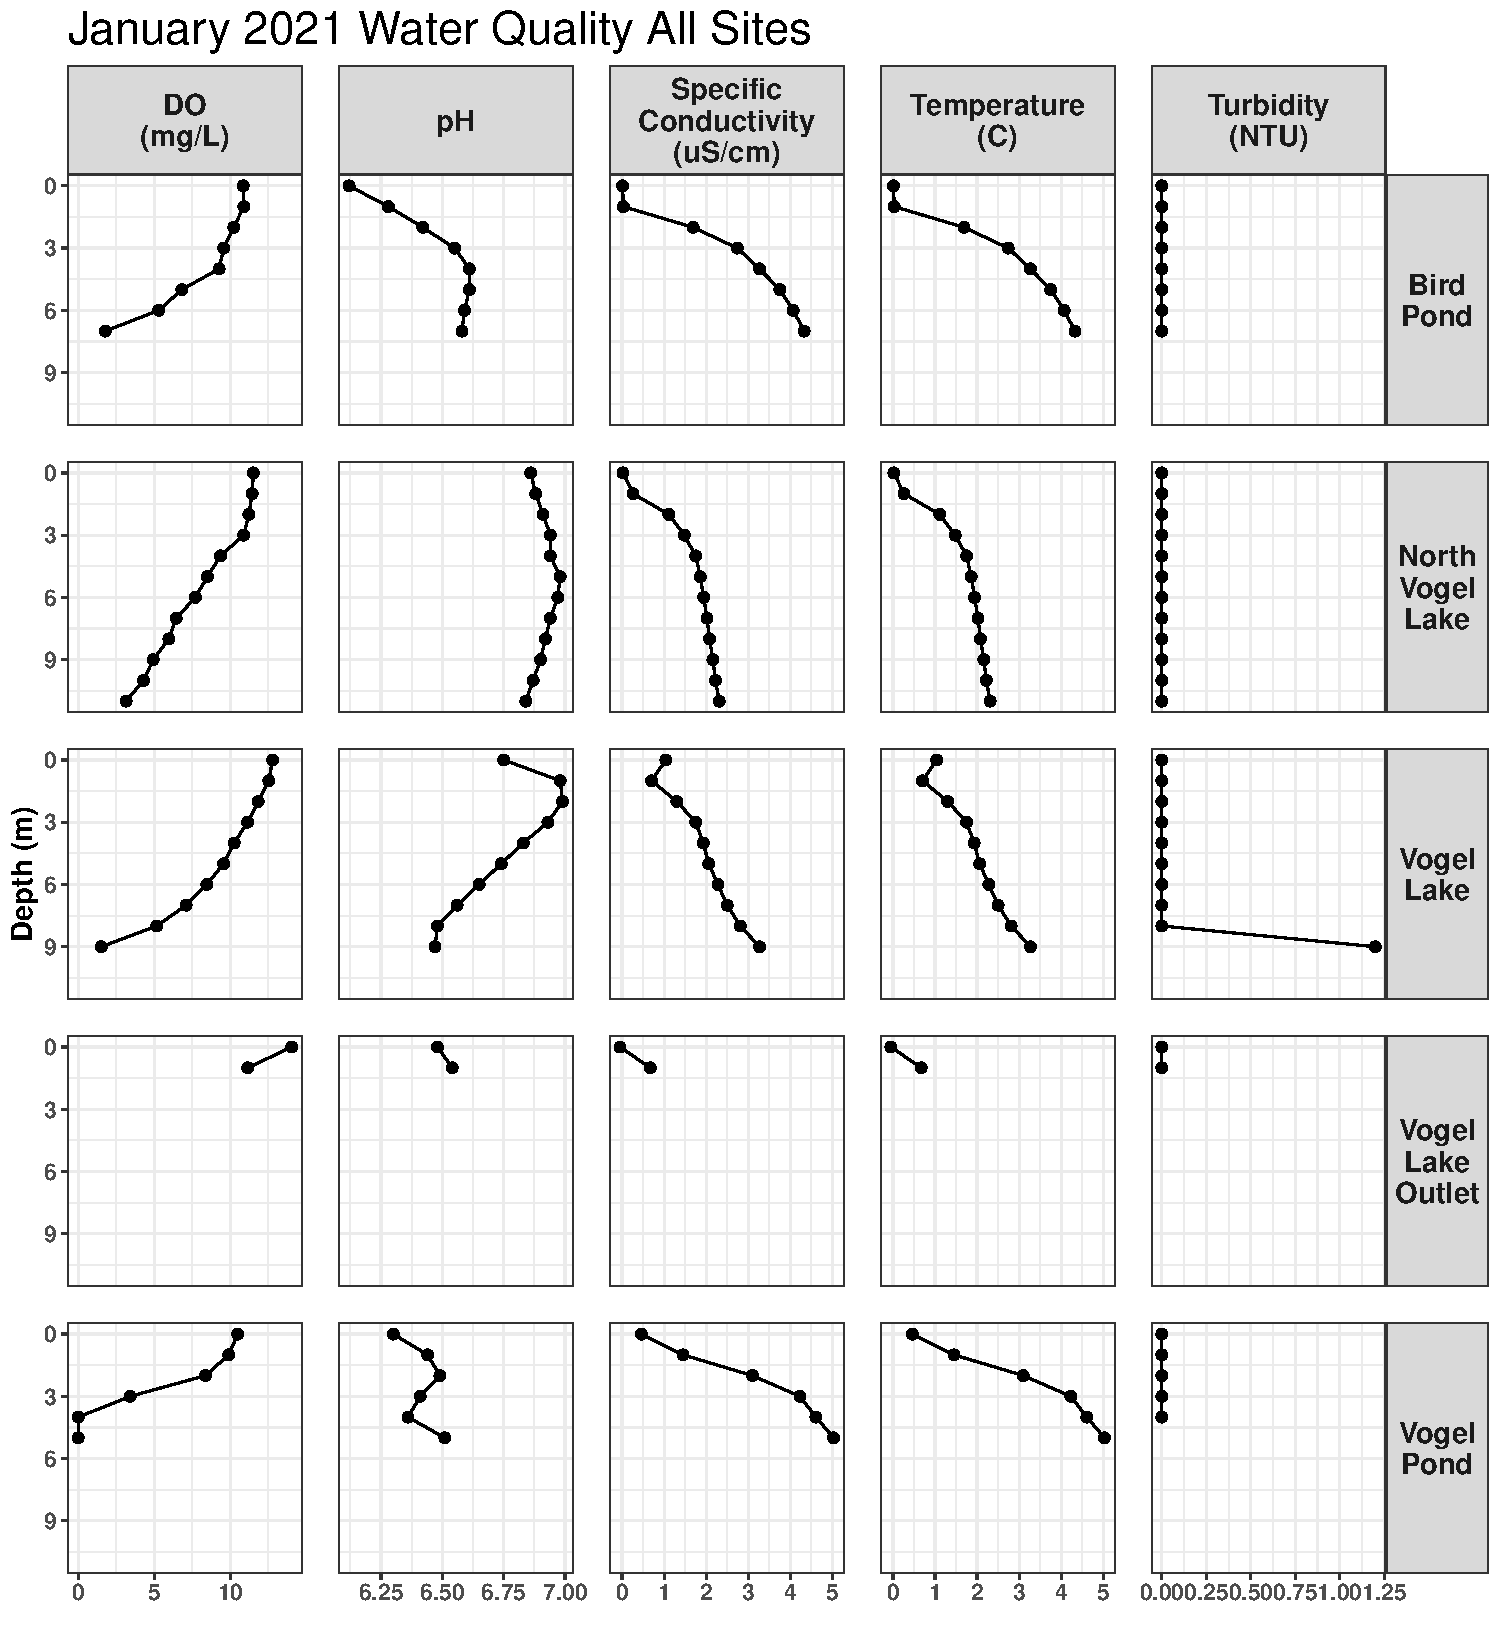
\includegraphics{Miller_Creek_Vogel_Lake_Water_Quality_files/figure-latex/jan21-wqx-1.pdf}
\caption{\label{fig:jan21-wqx}January 2021}
\end{figure}

\hypertarget{march-2021}{%
\subsection{March 2021}\label{march-2021}}

March 23, 2021

\begin{figure}
\centering
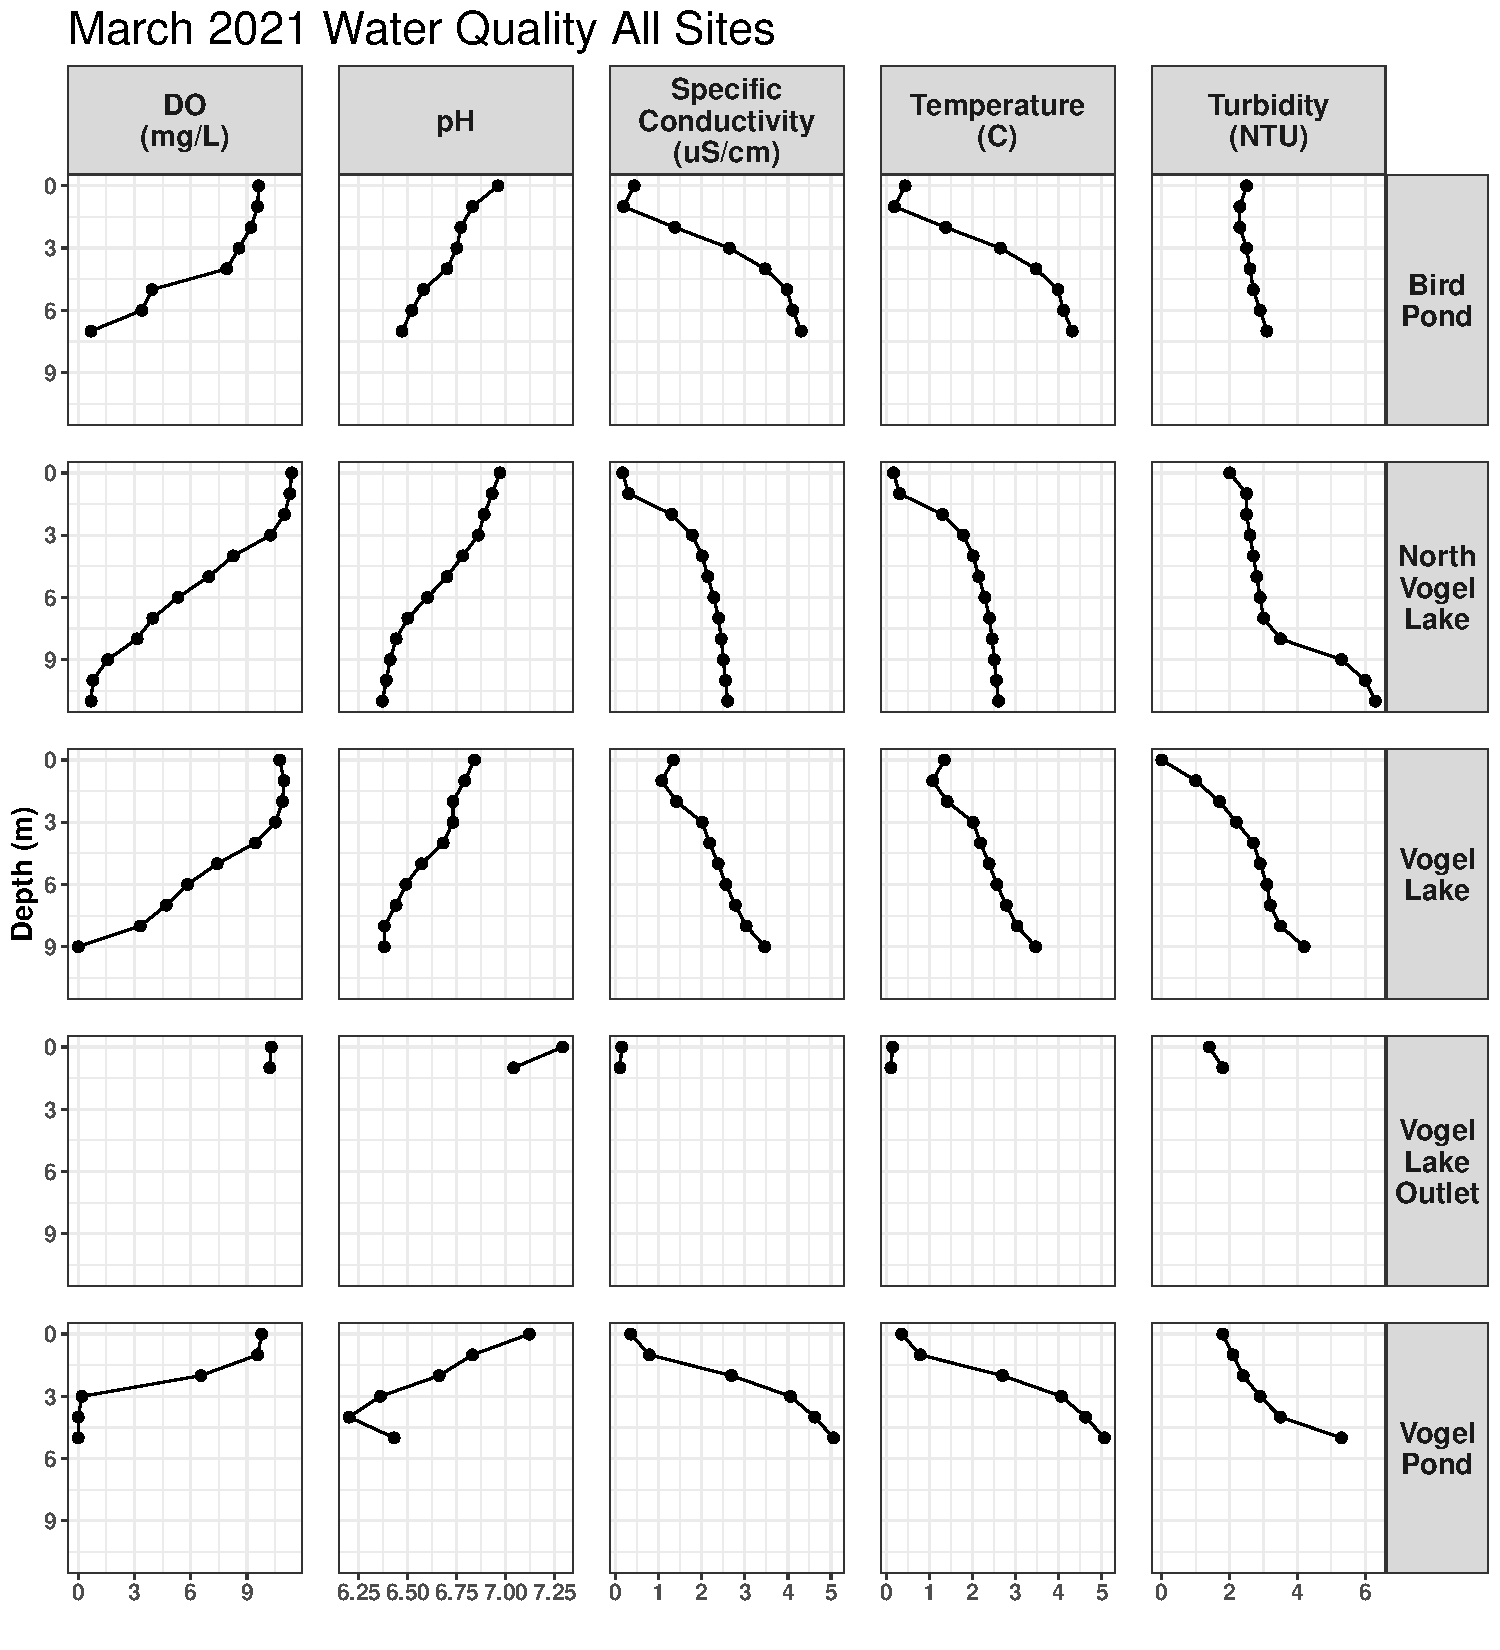
\includegraphics{Miller_Creek_Vogel_Lake_Water_Quality_files/figure-latex/unnamed-chunk-5-1.pdf}
\caption{\label{fig:unnamed-chunk-5}March 2021}
\end{figure}

\hypertarget{may-2021}{%
\subsection{May 2021}\label{may-2021}}

May 25, 2021

\begin{figure}
\centering
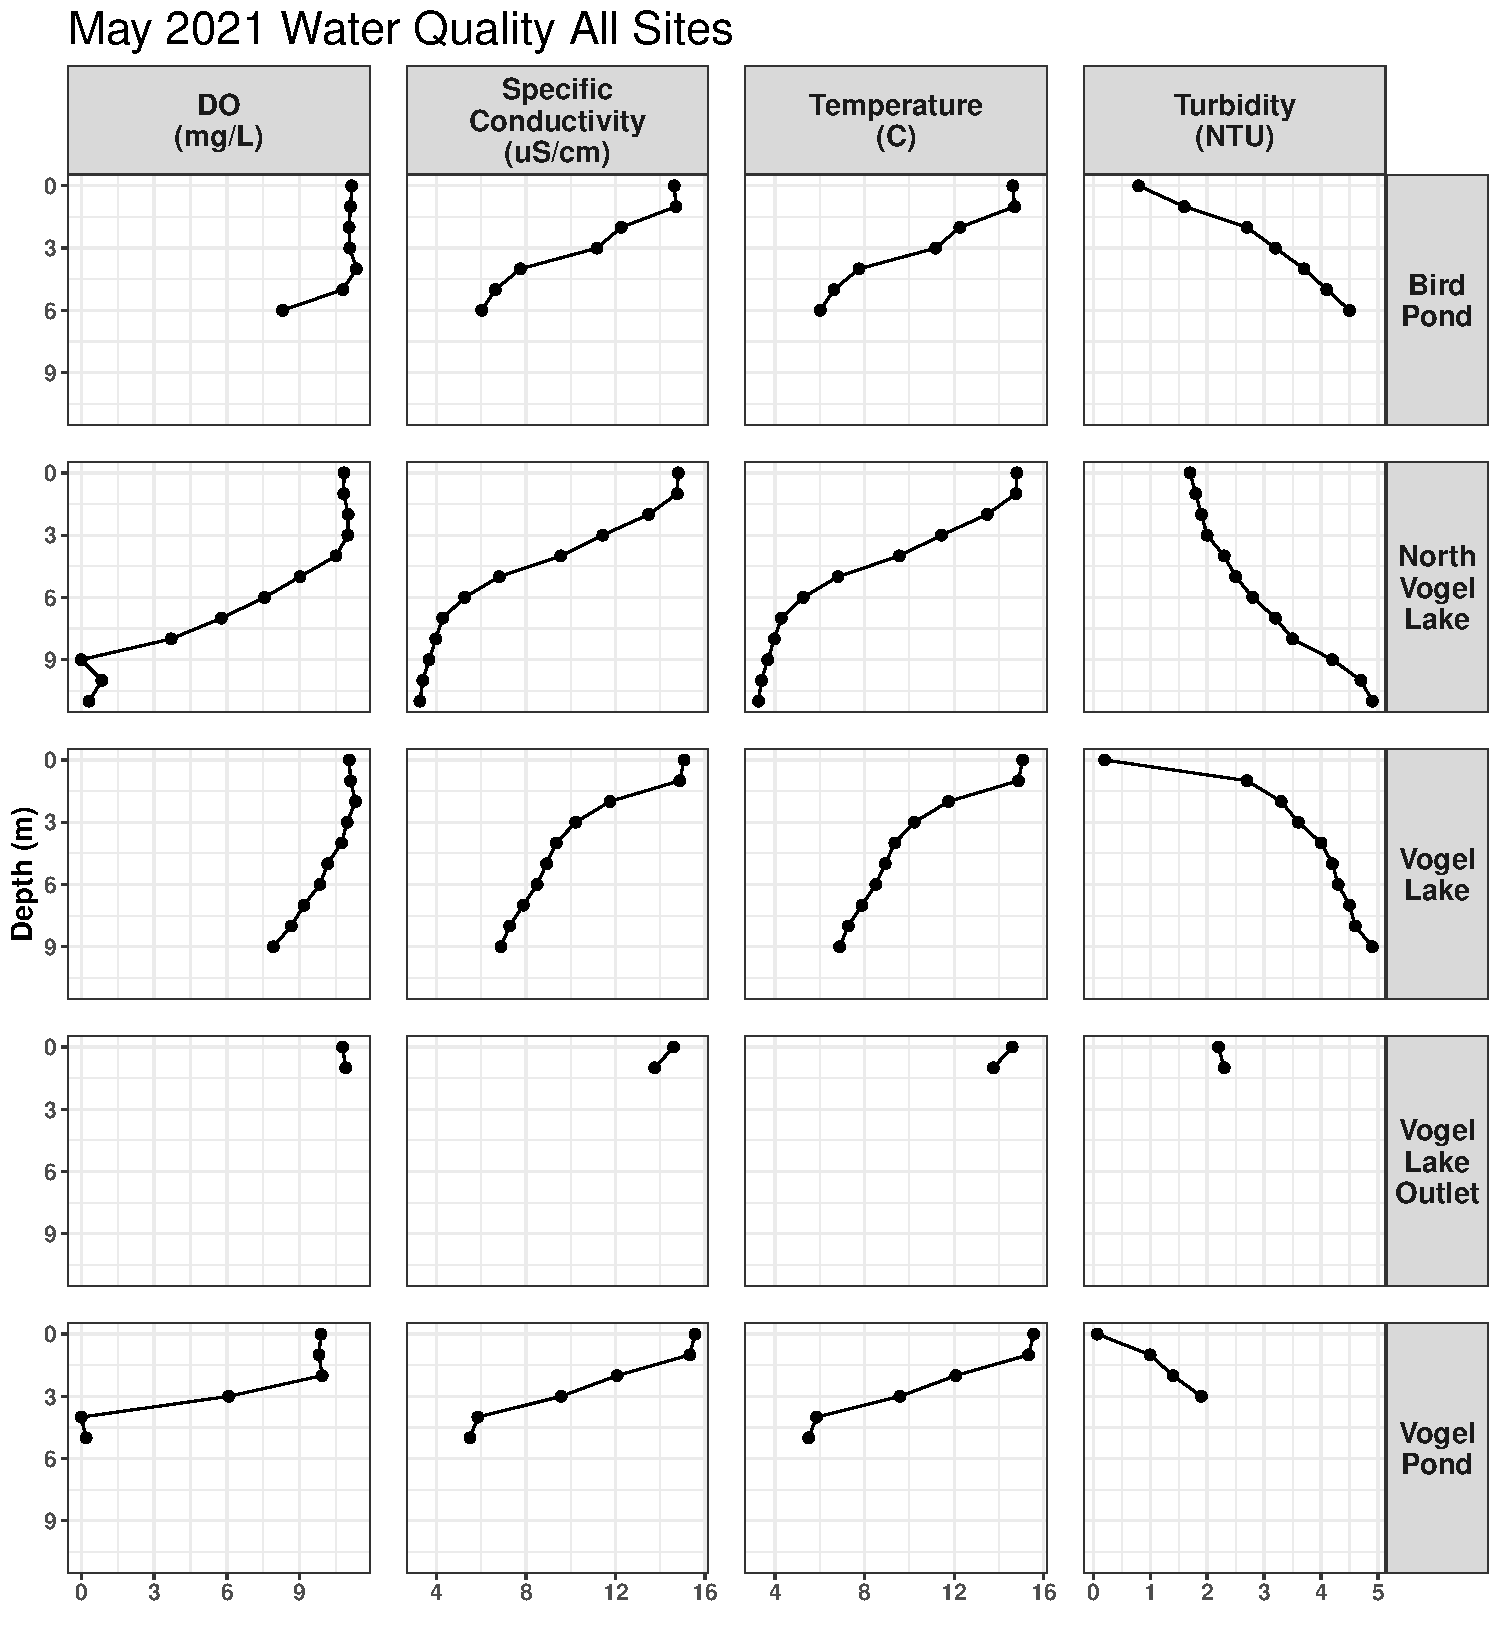
\includegraphics{Miller_Creek_Vogel_Lake_Water_Quality_files/figure-latex/unnamed-chunk-6-1.pdf}
\caption{\label{fig:unnamed-chunk-6}May 2021}
\end{figure}

\hypertarget{june-2021}{%
\subsection{June 2021}\label{june-2021}}

June 29, 2021

\begin{figure}
\centering
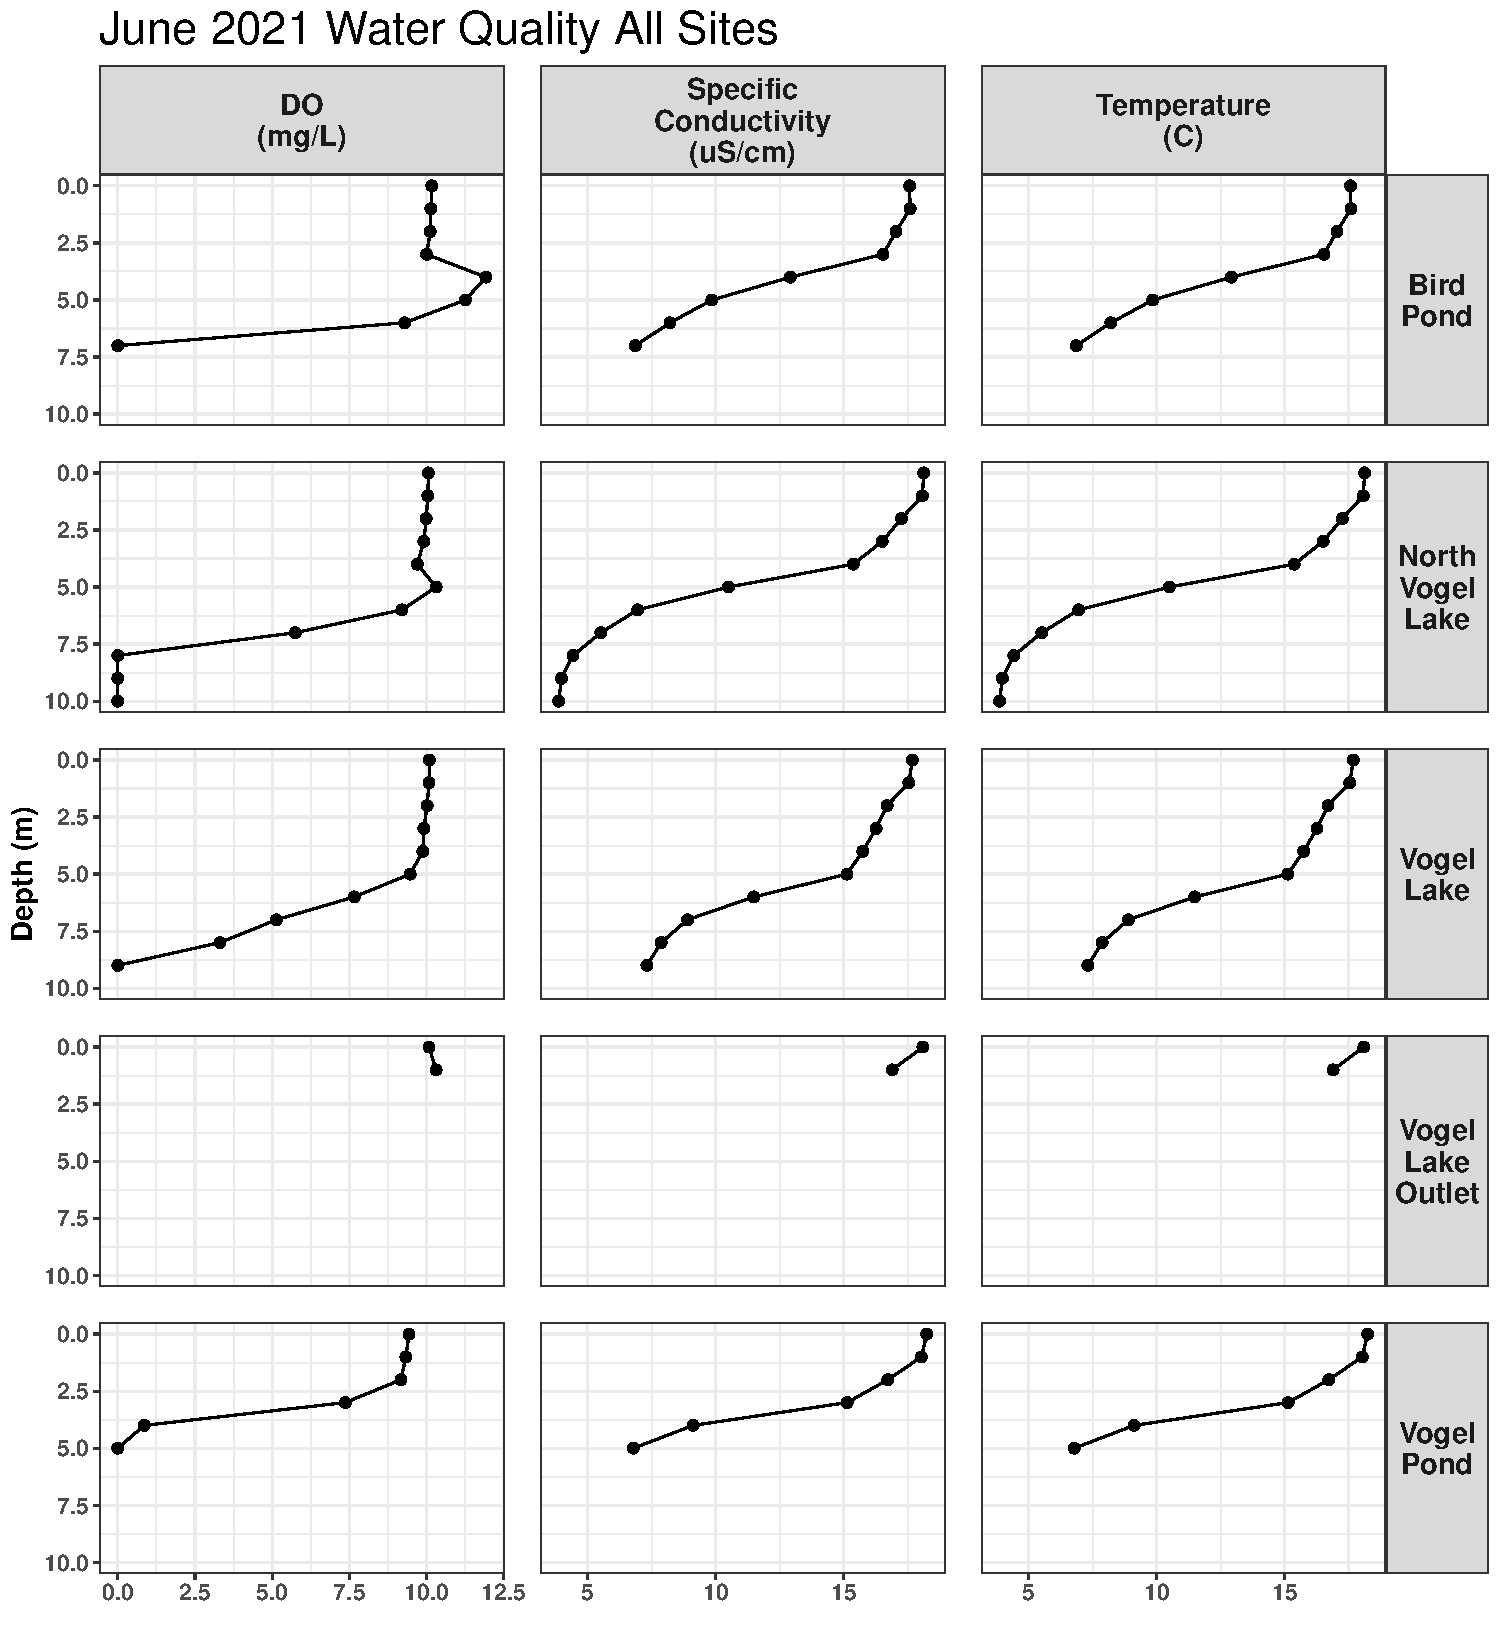
\includegraphics{Miller_Creek_Vogel_Lake_Water_Quality_files/figure-latex/unnamed-chunk-7-1.pdf}
\caption{\label{fig:unnamed-chunk-7}June 2021}
\end{figure}

Note: turbidity data is absent from June 2021 sampling due to an equipment issue.

\hypertarget{august-2021}{%
\subsection{August 2021}\label{august-2021}}

August 3, 2021

\begin{figure}
\centering
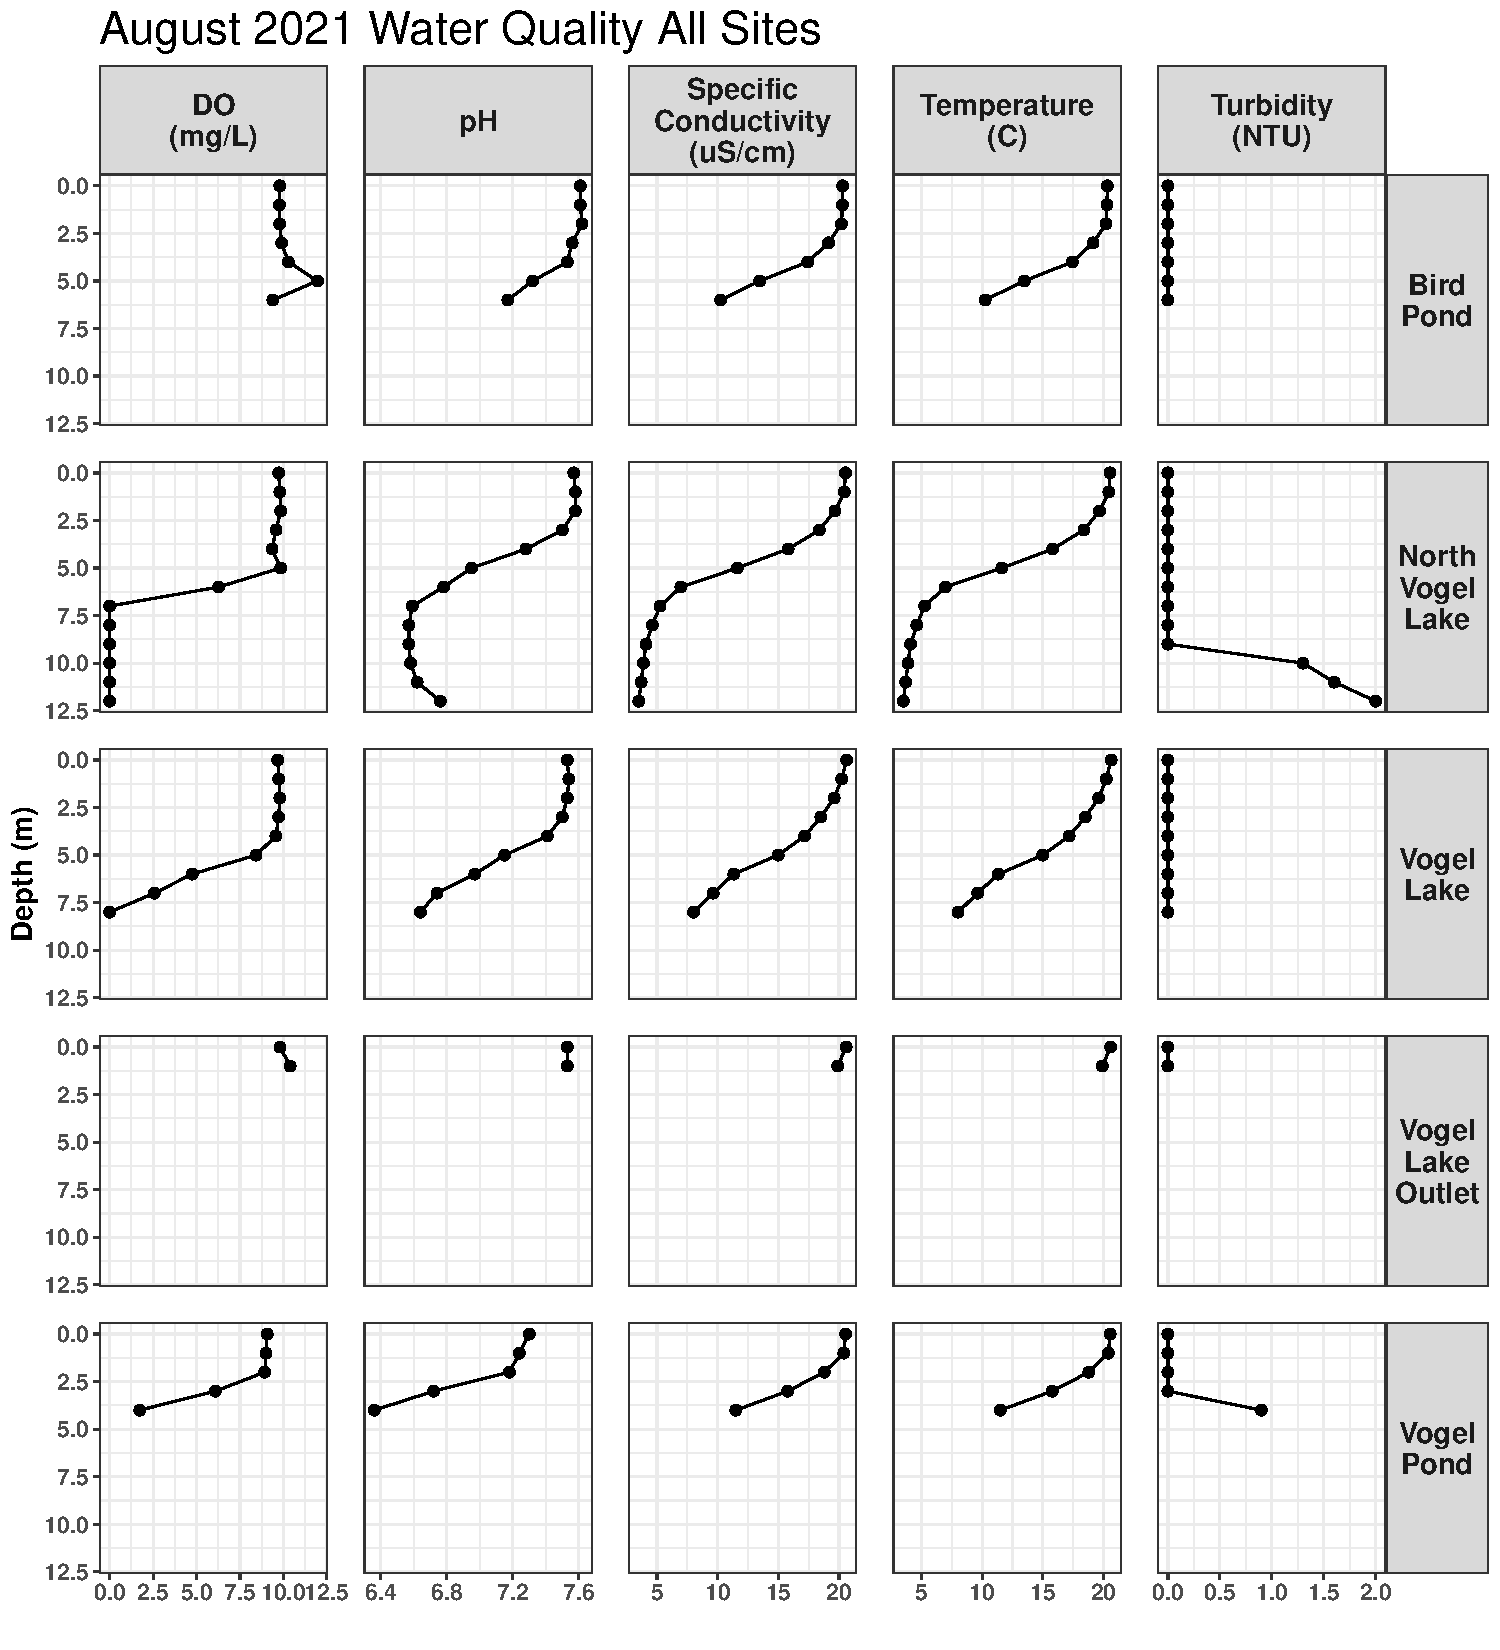
\includegraphics{Miller_Creek_Vogel_Lake_Water_Quality_files/figure-latex/unnamed-chunk-8-1.pdf}
\caption{\label{fig:unnamed-chunk-8}August 2021}
\end{figure}

\hypertarget{september-2021}{%
\subsection{September 2021}\label{september-2021}}

September 15, 2021

\begin{figure}
\centering
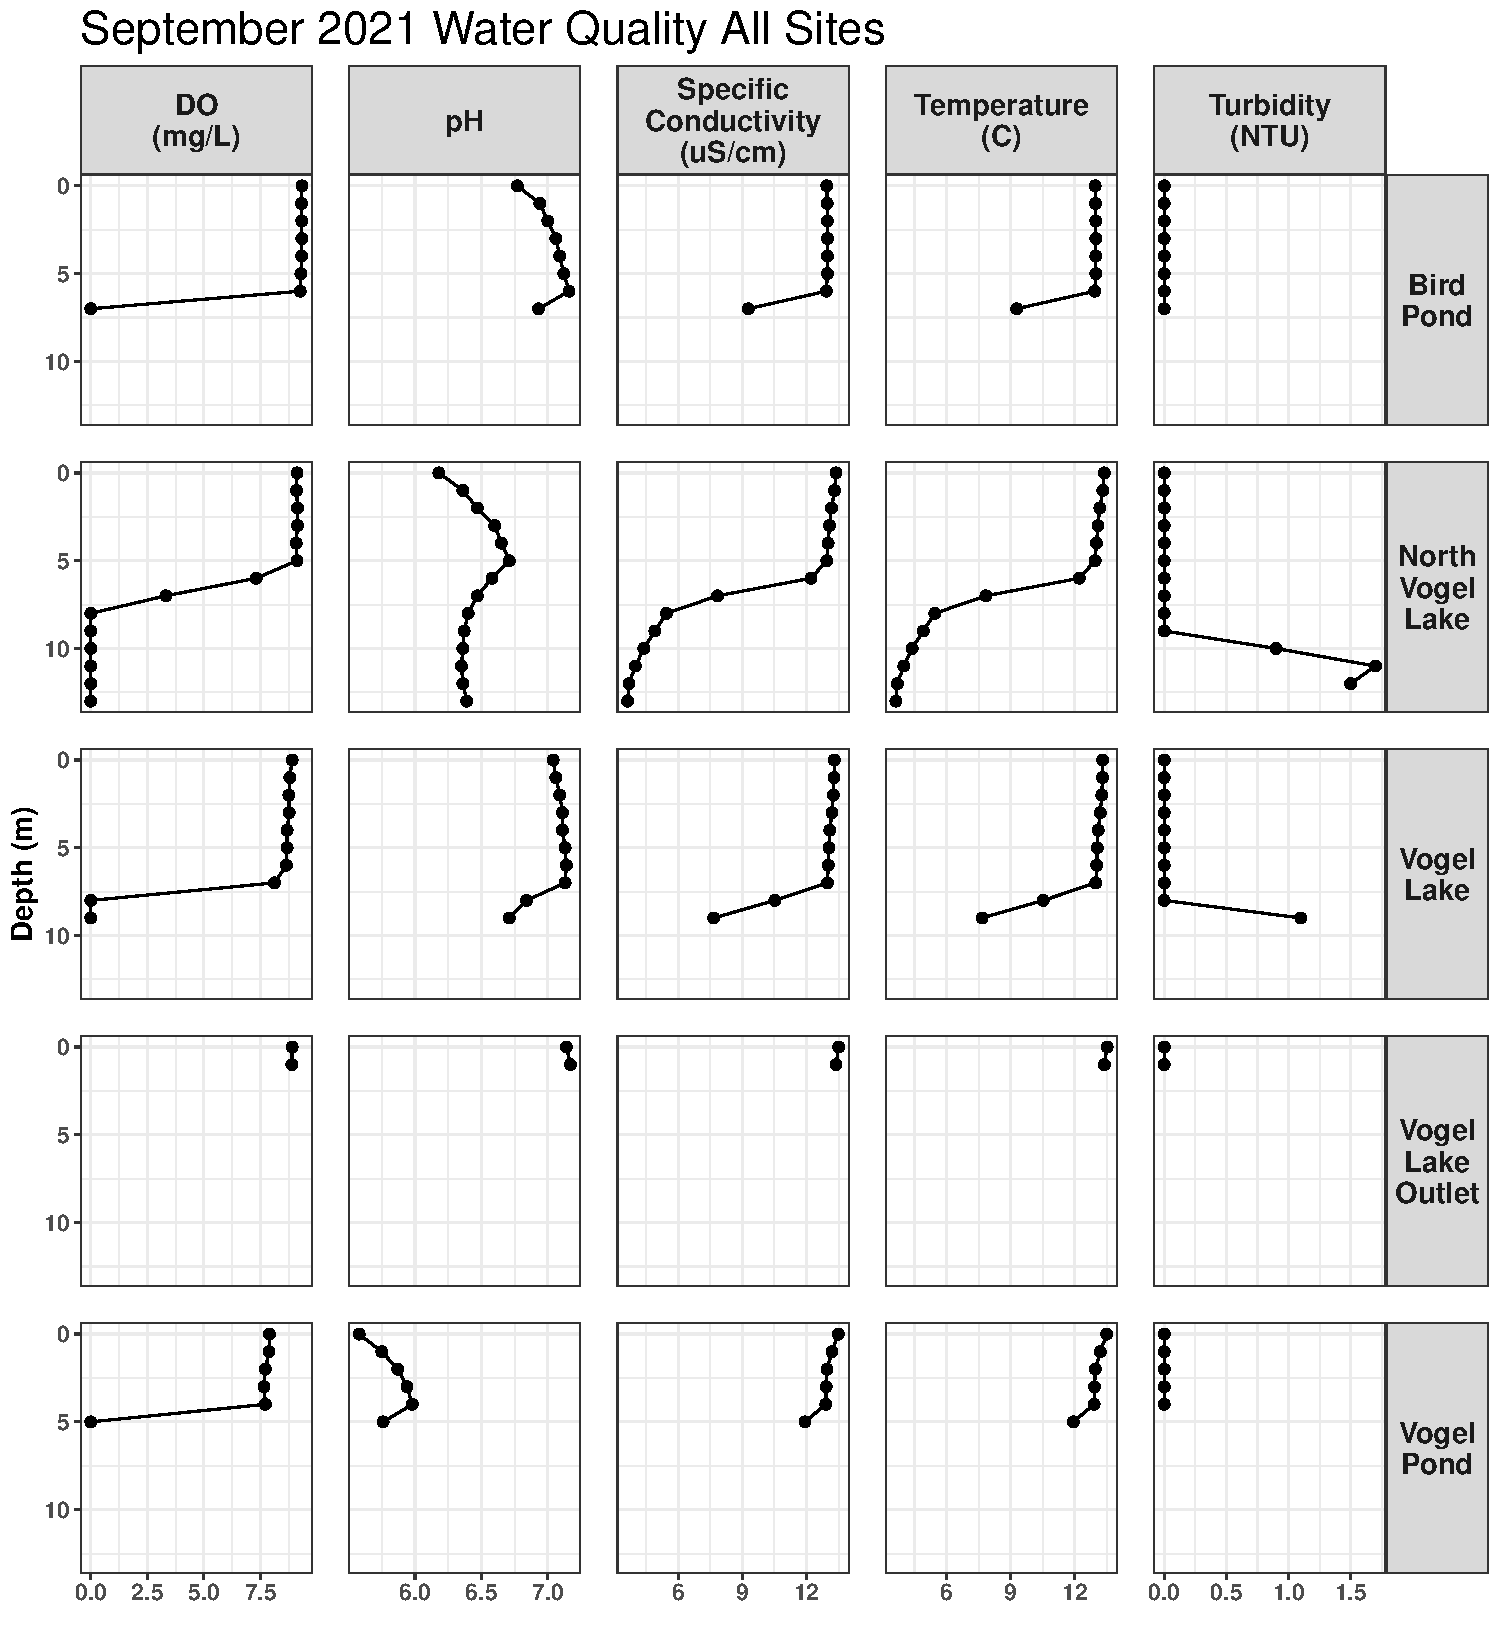
\includegraphics{Miller_Creek_Vogel_Lake_Water_Quality_files/figure-latex/unnamed-chunk-9-1.pdf}
\caption{\label{fig:unnamed-chunk-9}September 2021}
\end{figure}

\begin{center}\rule{0.5\linewidth}{0.5pt}\end{center}

\hypertarget{overall-data}{%
\section{Overall Data}\label{overall-data}}

\hypertarget{dissolved-oxygen}{%
\subsubsection{Dissolved Oxygen}\label{dissolved-oxygen}}

\begin{figure}
\centering
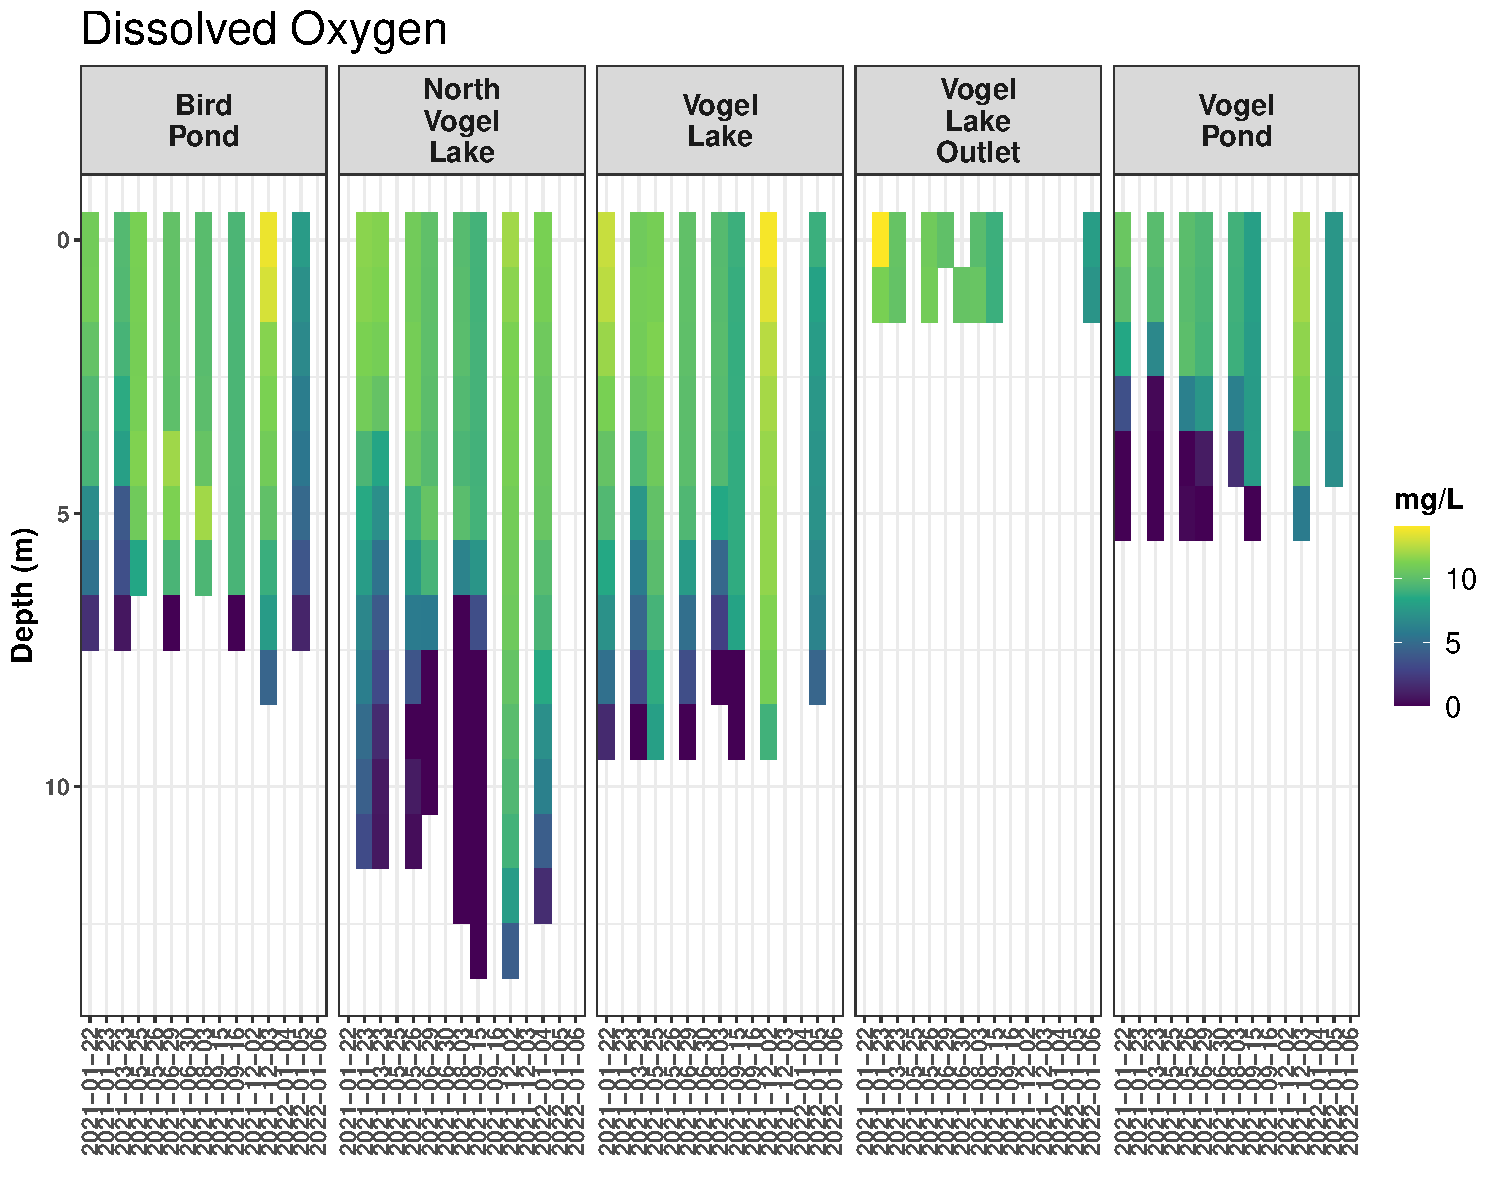
\includegraphics{Miller_Creek_Vogel_Lake_Water_Quality_files/figure-latex/unnamed-chunk-10-1.pdf}
\caption{\label{fig:unnamed-chunk-10}Dissolved Oxygen (mg/L)}
\end{figure}

\hypertarget{ph}{%
\subsubsection{pH}\label{ph}}

\begin{figure}
\centering
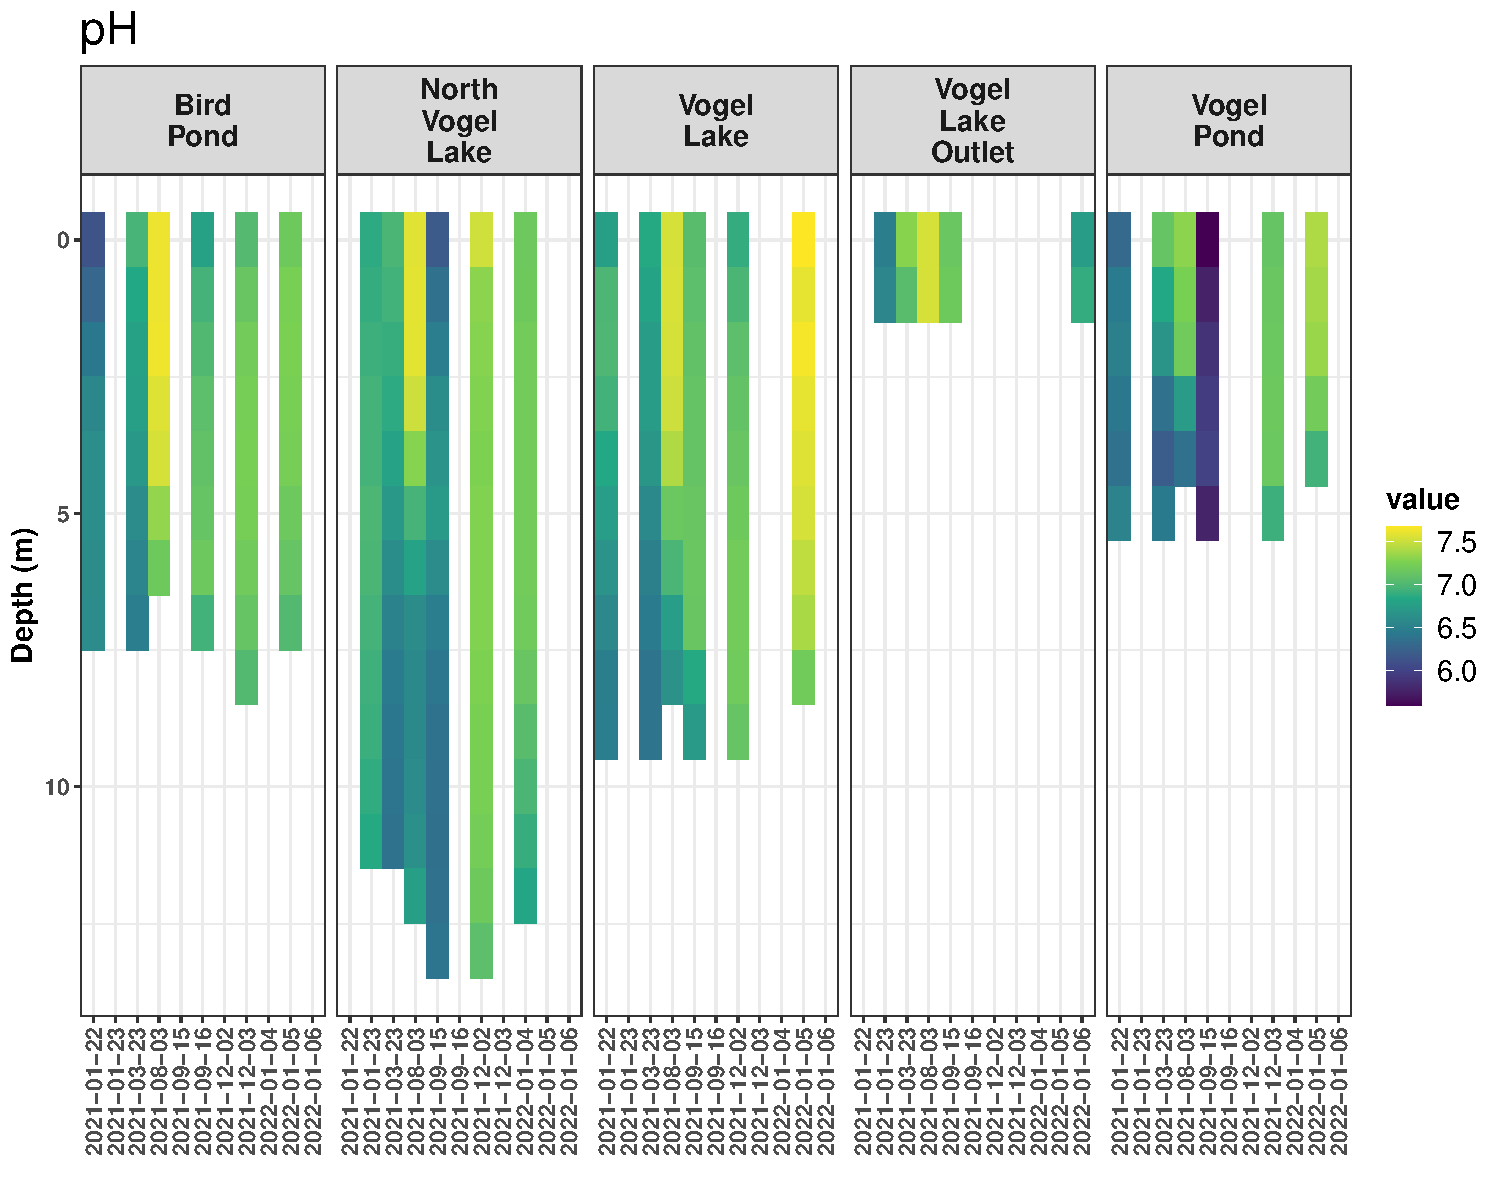
\includegraphics{Miller_Creek_Vogel_Lake_Water_Quality_files/figure-latex/unnamed-chunk-11-1.pdf}
\caption{\label{fig:unnamed-chunk-11}pH}
\end{figure}

Note: pH values are excluded from the May and June 2021 site visits due to an instrument error.

\hypertarget{turbidity}{%
\subsubsection{Turbidity}\label{turbidity}}

\begin{figure}
\centering
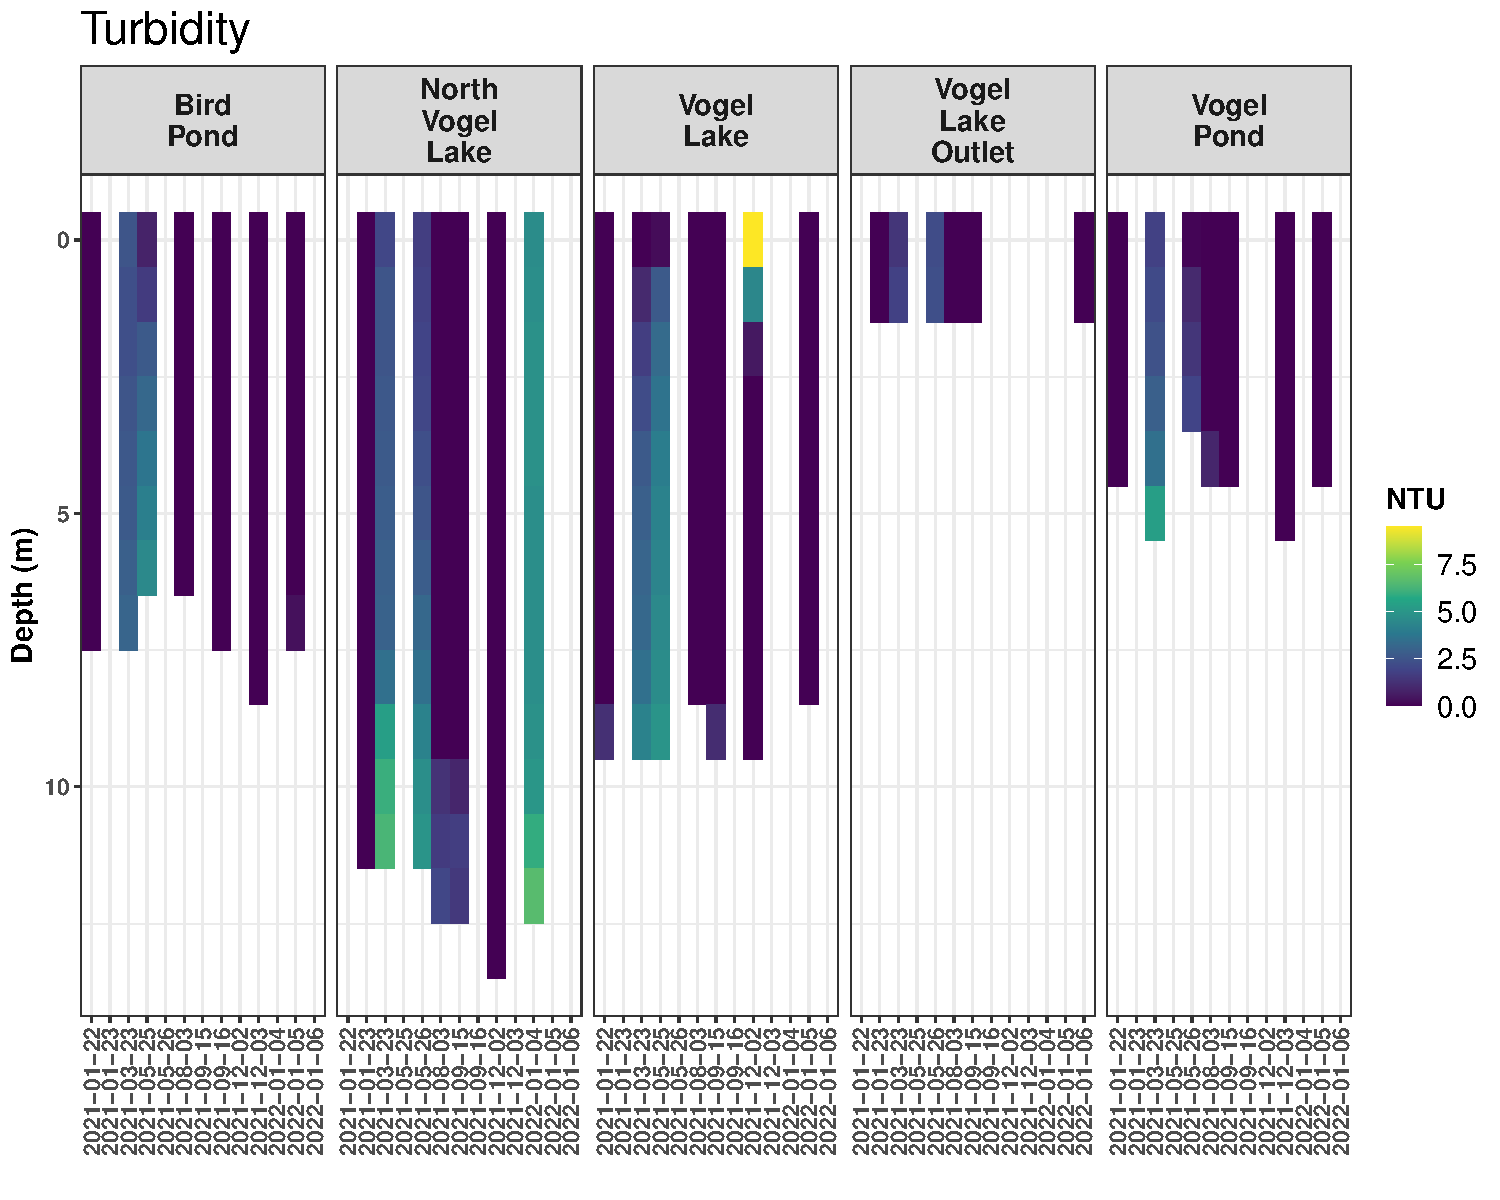
\includegraphics{Miller_Creek_Vogel_Lake_Water_Quality_files/figure-latex/unnamed-chunk-12-1.pdf}
\caption{\label{fig:unnamed-chunk-12}Turbidity (NTU)}
\end{figure}

Note: some turbidity values near the benthic surface of each site visit are not displayed in the above plot in order to improve visualization.

\hypertarget{conductivity}{%
\subsubsection{Conductivity}\label{conductivity}}

\begin{figure}
\centering
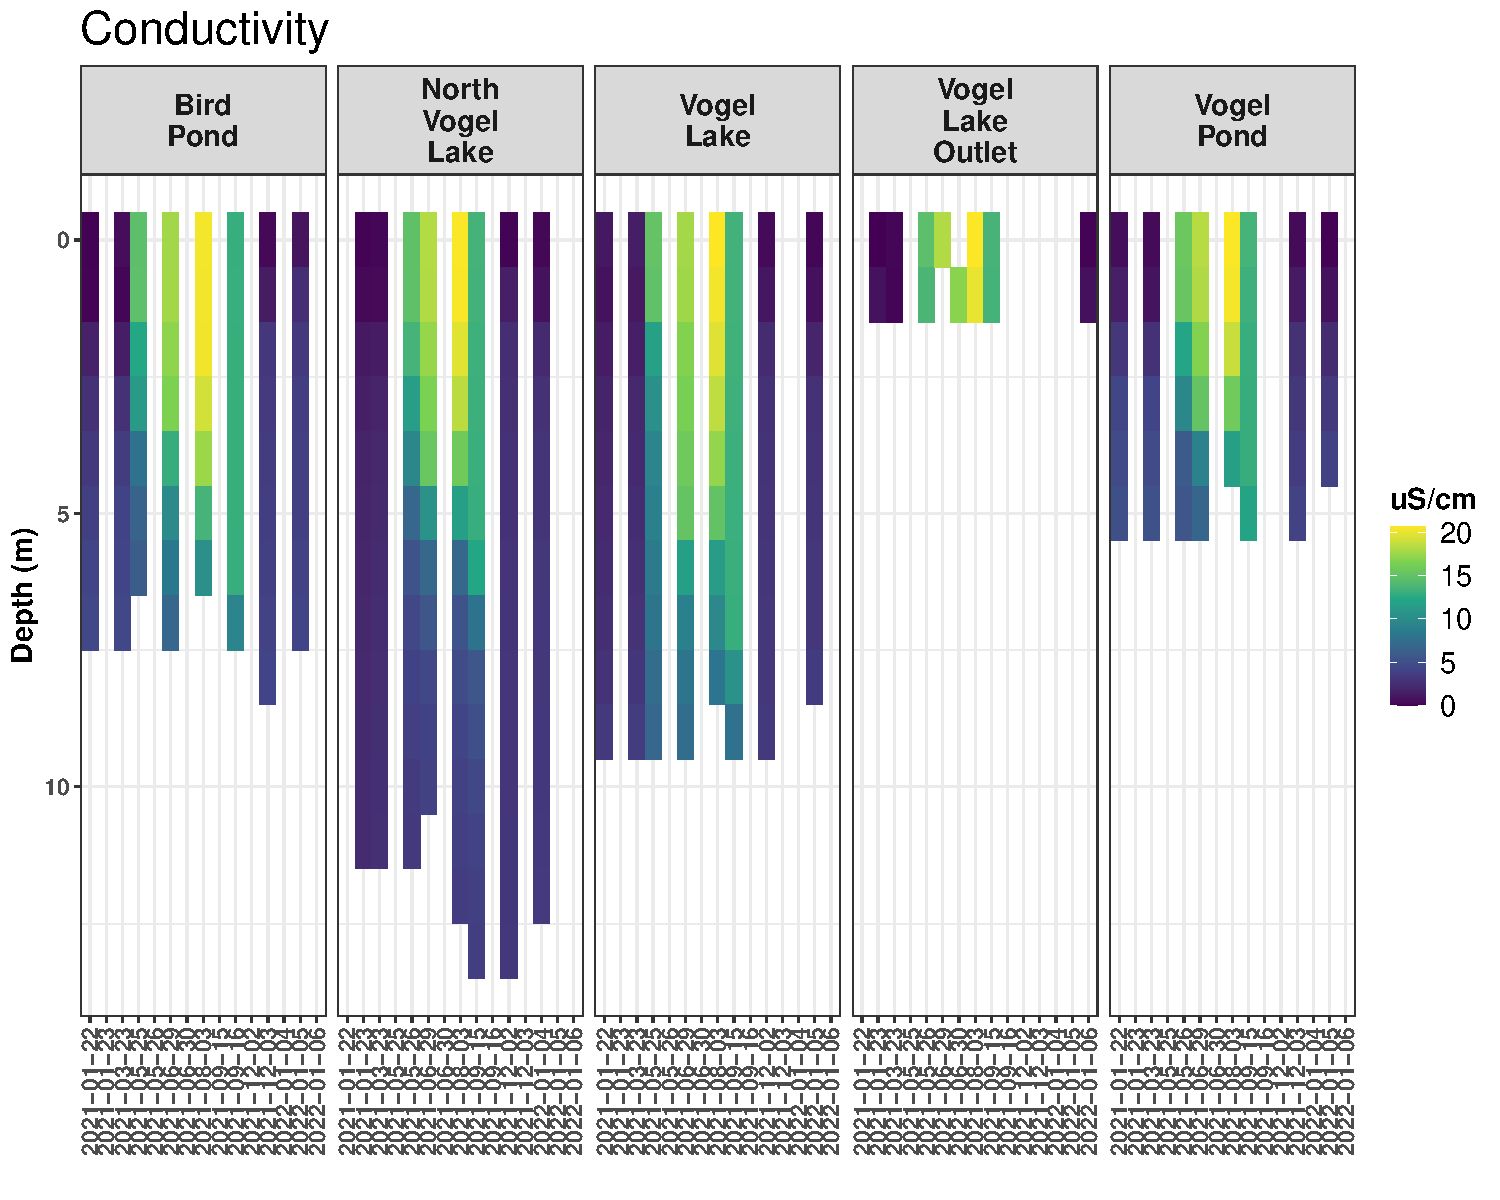
\includegraphics{Miller_Creek_Vogel_Lake_Water_Quality_files/figure-latex/unnamed-chunk-13-1.pdf}
\caption{\label{fig:unnamed-chunk-13}Conductivity (uS/cm)}
\end{figure}

\hypertarget{water-temperature}{%
\subsubsection{Water Temperature}\label{water-temperature}}

\begin{figure}
\centering
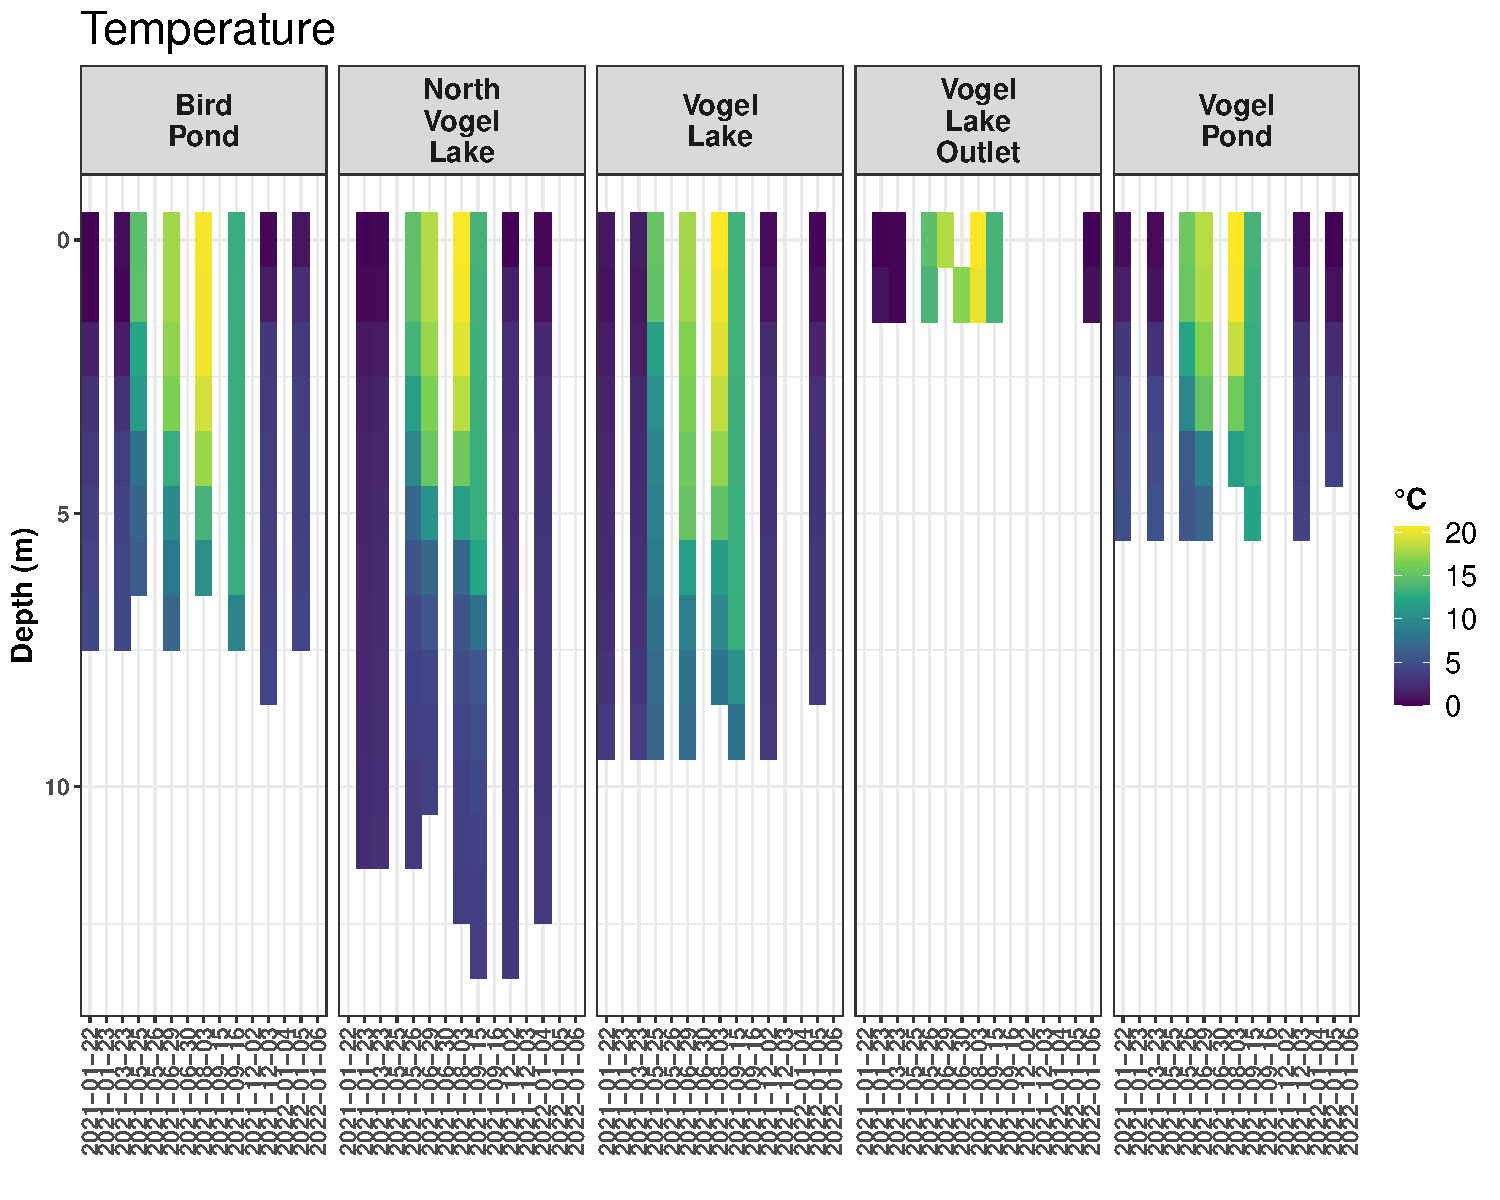
\includegraphics{Miller_Creek_Vogel_Lake_Water_Quality_files/figure-latex/unnamed-chunk-14-1.pdf}
\caption{\label{fig:unnamed-chunk-14}Water Temperature (C)}
\end{figure}

\begin{center}\rule{0.5\linewidth}{0.5pt}\end{center}

\hypertarget{site-summaries}{%
\section{Site Summaries}\label{site-summaries}}

A table of summary statistics for water quality parameters at each site will be provided here.

\hypertarget{miller-creek-discharge-flow-rate}{%
\chapter{Miller Creek Discharge \& Flow Rate}\label{miller-creek-discharge-flow-rate}}

\hypertarget{introduction-1}{%
\subsection{Introduction}\label{introduction-1}}

Hydrology fieldwork focusing on flow and discharge is being conducted throughout the Miller Creek drainage in Fall 2020 - Spring 2021.

\begin{itemize}
\item
  Near the mouth of Miller Creek, a discharge measurement station was installed in October 2020. At this site a pressure transducer measures water level, and discharge measurements are collected periodically using an Acoustic Doppler Velocimeter. These data, along with staff plate observations, are being used to create a rating discharge curve.
\item
  An experiment to study stream flow rate in Miller Creek was conducted September 15-17, 2021. A plug of dissolved salt (NaCl) was discharged in to the creek, and the resultant spike in conductivity was observed downstream 0.64 km stream distance.
\end{itemize}

Raw water quality field data is stored in a Google Sheet that can be viewed at \url{https://tinyurl.com/kwf-vogel-wqx-data} under the ``Discharge Measurements'' tab.

Site photos are available through a point-and-click pop-up map at \url{https://arcg.is/0fqvb0}.

\hypertarget{miller-creek-discharge-rating-curve}{%
\subsection{Miller Creek Discharge Rating Curve}\label{miller-creek-discharge-rating-curve}}

A discharge station was established in October 2020 near the mouth of Miller Creek, including a staff plate and pressure transducer.

Site visits have been made opportunistically depending on precipitation throughout Summer/Fall 2021. At each site visit, the pressure transducer is downloaded and a discharge measurement is collected using a SondeTek Flowtracker. See Figure \ref{fig:rating-curve} for the discharge rates and staff plate values observed to date.

Once a minimum of eight discharge measurements are available in Fall 2021, a curve will be fit to the scatter plot of stage height vs.~discharge. This relationship will be used in conjunction with pressure transducer data to create a flow hydrograph.

\begin{figure}
\centering
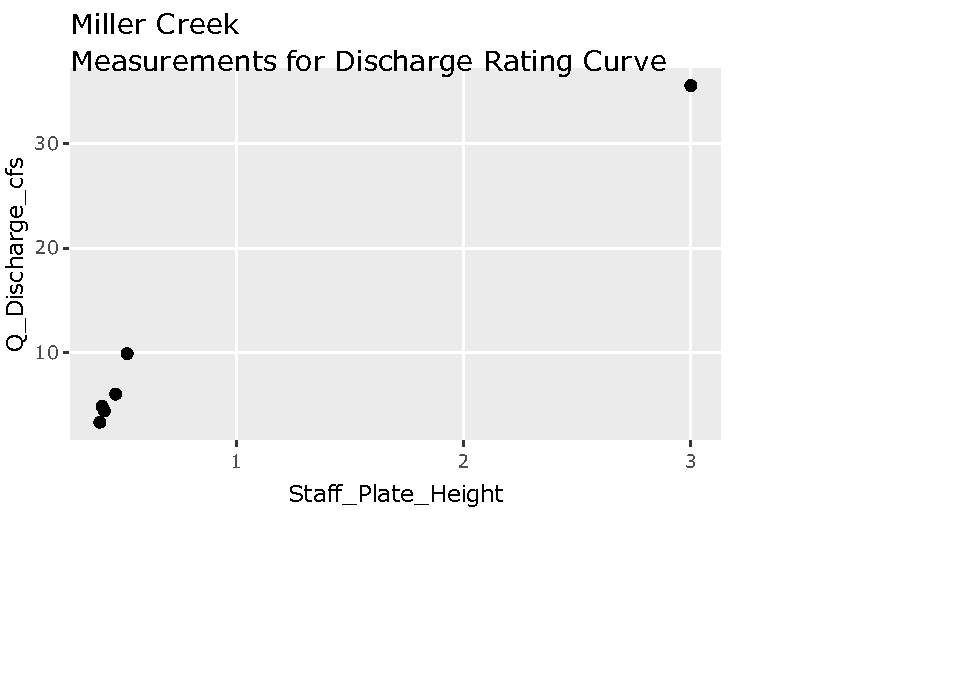
\includegraphics{Miller_Creek_Vogel_Lake_Water_Quality_files/figure-latex/rating-curve-1.pdf}
\caption{\label{fig:rating-curve}Measurements for Miller Creek Discharge Rating Curve}
\end{figure}

\hypertarget{discharge-measurements-at-other-sites}{%
\subsection{Discharge measurements at other sites}\label{discharge-measurements-at-other-sites}}

Additional discharge measurements were taken throughout Summer 2021 at two additional sites near Vogel Lake, near the outlets of Kuguyuk Pond and Bird Pond. See Figure \ref{fig:other-discharge} for discharge values observed to date.

\begin{figure}
\centering
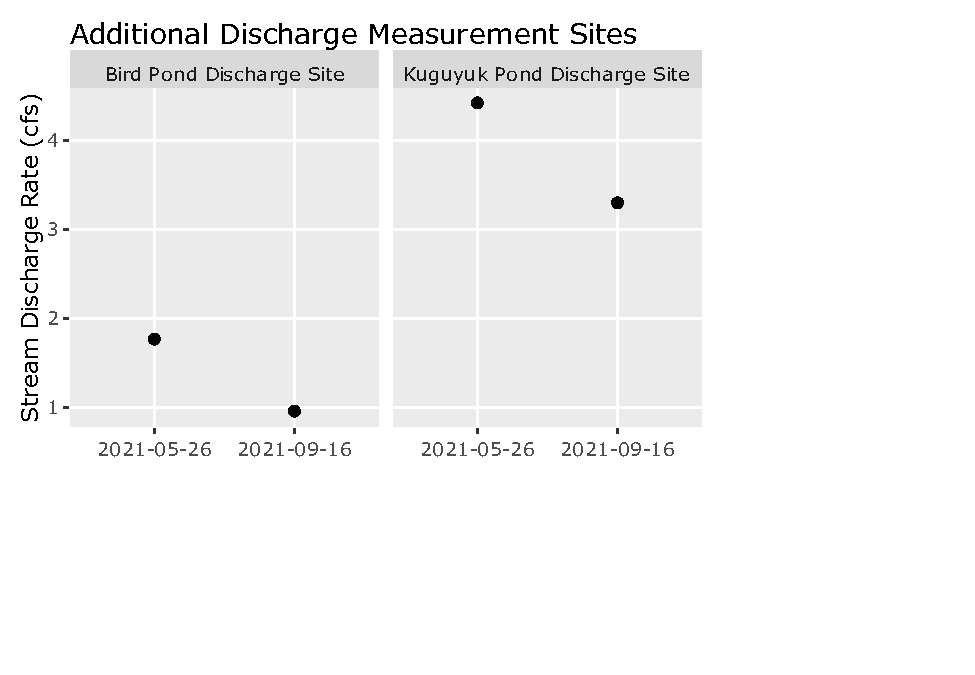
\includegraphics{Miller_Creek_Vogel_Lake_Water_Quality_files/figure-latex/other-discharge-1.pdf}
\caption{\label{fig:other-discharge}Other discharge measurements}
\end{figure}

\hypertarget{pressure-transducer-data}{%
\subsection{Pressure Transducer Data}\label{pressure-transducer-data}}

Work in progress here 8/10/2021

\hypertarget{stream-flow-rate-experiment}{%
\subsection{Stream Flow Rate Experiment}\label{stream-flow-rate-experiment}}

On September 15-17, 2021 we conducted an experiment to examine stream flow rate in Miller Creek. We measured downstream transport time of dissolved solutes by deploying a plug of dissolved salt and measuring a resultant change in conductivity at a site downstream.

\hypertarget{methods}{%
\paragraph{Methods}\label{methods}}

We deployed a plug of dissolved salt into the Miller Creek stream channel and measured conductivity continuously at a downstream site. See Figure \ref{fig:nacl-map} for salt deployment and conductivity monitoring sites.

\begin{figure}
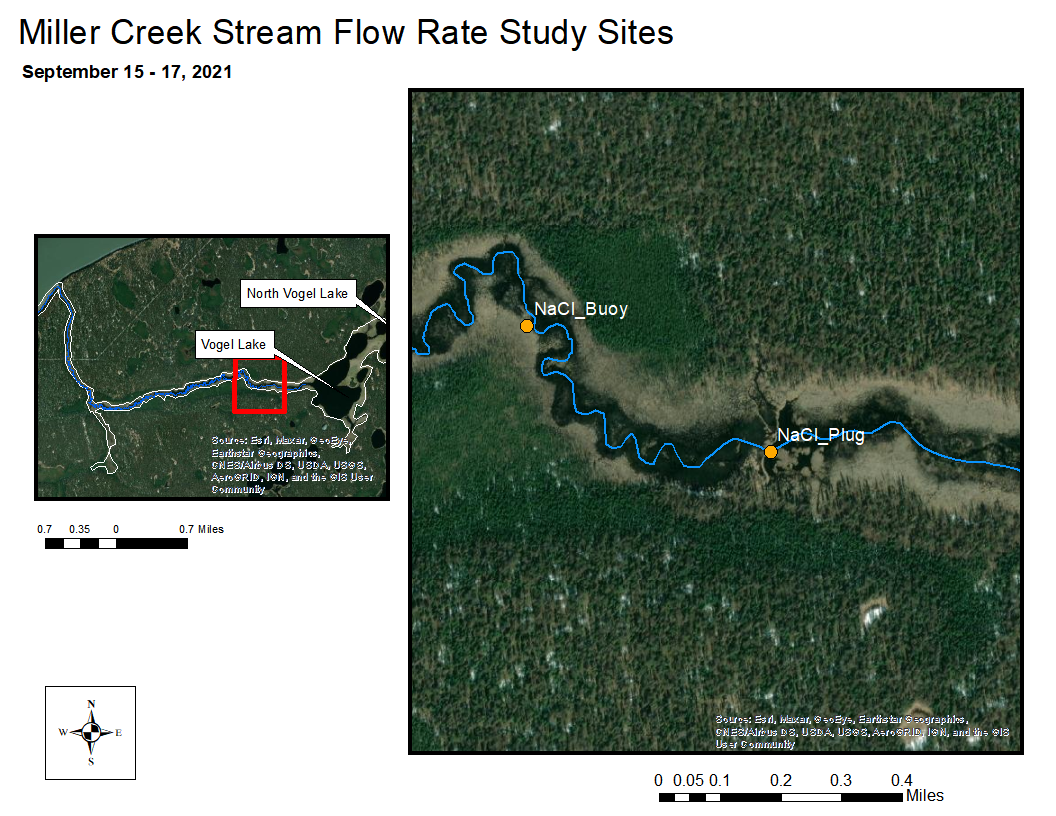
\includegraphics[width=14.67in]{images/stream_flow_rate_sites} \caption{Stream Flow Rate Study Area. Stream distance between the NaCl release site and the downstream measurement site is 0.63 km (0.39 mi).}\label{fig:nacl-map}
\end{figure}

The Vogel Lake / Miller Creek system is a low-gradient drainage with little observable flow within 0.5 miles downstream of the lake outlet. We deployed our salt plug downstream from the Vogel Lake outlet at the first site with visibly evident surface flow, which was over the top of the first downstream beaver dam.

We released 140 lbs of dissolved NaCl by dissolving appx 15 lbs at a time in a 35 gallon trash can, then discharging it on the downstream side of the beaver dam into the stream channel. Our downstream site monitoring conductivity was 0.63 km (0.39 mi) downstream center-channel.

To record conductivity we used a pair of simultaneously deployed Hydrolab MS5 Sondes suspended from a floating buoy. We programmed the sondes to record at 0.25 hour intervals. We examined the resultant time series for exposure or errors and removed these data points. We averaged conductivity values between the two Hydrolab units in the final results.

\hypertarget{results}{%
\paragraph{Results}\label{results}}

We measured a readily evident rise in conductivity values at the downstream monitoring site. See Figure \ref{fig:nacl-fig} for the time series of conductivity data.

\begin{figure}
\centering
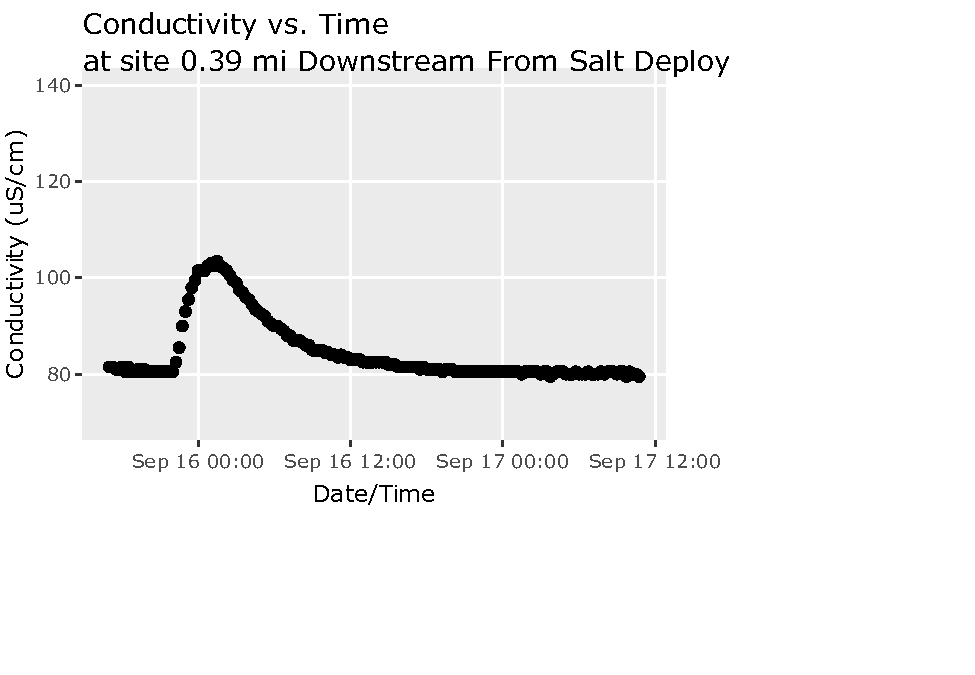
\includegraphics{Miller_Creek_Vogel_Lake_Water_Quality_files/figure-latex/nacl-fig-1.pdf}
\caption{\label{fig:nacl-fig}Conductivity values at the site downstream of the NaCl release site. The NaCl plug was released at 19:30 on 9/15/2021. The release and measurement site coordinates can be accessed at the ArcGIS Online Map at \url{https://arcg.is/0LqOKH0}.}
\end{figure}

In Figure \ref{fig:nacl-fig} we can observe the following:

\begin{itemize}
\item
  \underline{Initial NaCl Deployment:} 9/15/2021 19:30
\item
  \underline{Start of the rising limb of the conductivity spike:} 9/15/2021 22:00 (2.5 hrs after deployment)
\item
  \underline{Maximum conductivity peak (\textasciitilde20\% above baseline values):} 01:30 9/16/2021 (6.0 hours after deployment)
\item
  \underline{Return to baseline conductivity levels:} 9/16/2021 15:00 (19.5 hrs after deployment)
\end{itemize}

Based on these results, peak concentration of the dissolved solute traveled though this section of Miller Creek at \underline{\textbf{0.11 km/h (0.06 mph)}}.

\hypertarget{watershed-mapping}{%
\chapter{Watershed Mapping}\label{watershed-mapping}}

\begin{itemize}
\item
  Watershed mapping efforts for this project include a combination of on the ground fieldwork and GIS based approaches.
\item
  An ArcGIS Online interactive map outlining fieldwork sites and associated results is found at the following link: \url{https://arcg.is/0Djmay}
\item
  Technicians walked the Miller Creek corridor on foot on May 27-28, 2021 to identify hydrologic features that may be difficult to identify from the air, such as seepages. The locations are visible in the ArcGIS Online map in the ``Hydrologic Connectivity'' layer, and may be downloaded here as .gpx files:

  \begin{itemize}
  \item
    All hydrologic features (n = 67): \href{https://drive.google.com/file/d/1PQu1v6nTD6MB3YStwBF3mgV0wydKziIa/view?usp=sharing}{miller\_creek\_features.gpx}
  \item
    Only seepage hydrologic features (n = 16): \href{https://drive.google.com/file/d/1_c4FQDR0t2sW_yphFuuiSpRmydPzjR3i/view?usp=sharing}{miller\_creek\_seepage\_features.gpx}
  \end{itemize}
\end{itemize}

\href{https://arcg.is/1GeLTX}{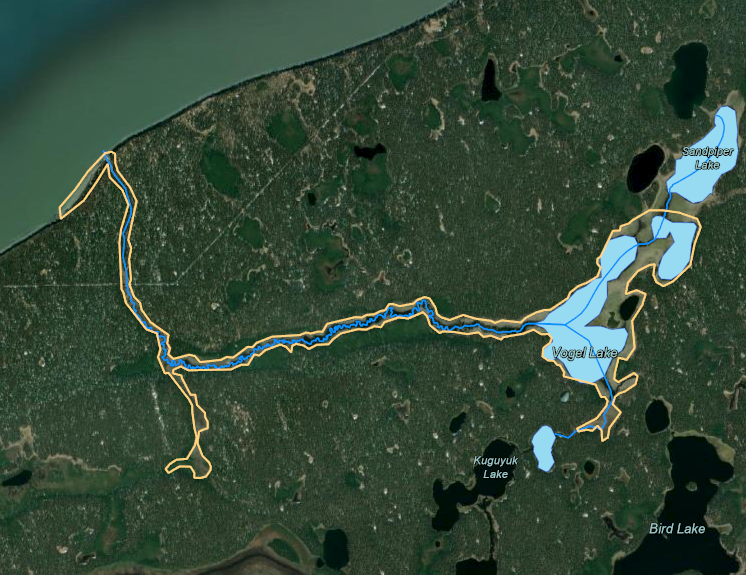
\includegraphics[width=5.20833in,height=\textheight]{images/miller_map.png}}

\hypertarget{fish-rescue}{%
\chapter{Fish Rescue}\label{fish-rescue}}

\hypertarget{summary}{%
\section{Summary}\label{summary}}

On September 27-29, 2021, staff from Kenai Watershed Forum and Cook Inlet Aquaculture Association led fish rescue efforts in Lower Miller Creek prior to rotenone treatment. We used minnow traps to capture juvenile fish, which were later transported by helicopter to Bird Pond for winter residency until post-treatment rotenone levels decrease to safe levels. A fish barrier currently at the outlet of Bird Pond will be removed in Summer 2022 pending confirmation of safe conditions.

\hypertarget{methods-1}{%
\section{Methods}\label{methods-1}}

We captured juvenile fish in the segment of Miller Creek extending from it's mouth at Cook Inlet to a location upstream approximately 1.3 km from the mouth, N 60.99530, W -150.50760.

We used Gee minnow traps baited with cured, disinfected salmon eggs. We placed eggs placed inside perforated canisters to prevent consumption by the fish. We placed minnow traps in locations known to be preferred by juvenile salmonids, including areas with woody debris, pools, and areas with riparian cover. We deployed traps for time periods of 6-12 hours at a time, and returned with all captured fish in five-gallon buckets to a central location. We identified all captured fish to genus or species for the purpose of ensuring that no juvenile pike were included in the captured population.

After identifying fish taxa, we stored juvenile fish in three perforated five gallon buckets submerged within the creek on site. We placed stones at the bottom of each bucket to keep them submerged. These fish were stored until being retrieved by helicopter for transport to Bird Lake on 10/1/2021.

\hypertarget{results-1}{%
\section{Results}\label{results-1}}

\begin{table}

\caption{\label{tab:rescue-tbl}Minnow trap deployment and fish capture, estimated data from Lower Miller Creek}
\centering
\begin{tabular}[t]{l|l|r|r}
\hline
Deployment\_Date\_Time & Retrieval\_Date\_Time & Trap\_Count & Fish\_Capture\\
\hline
2021-09-27 18:15:00 & 2021-09-28 10:00:00 & 48 & 400\\
\hline
2021-09-28 12:00:00 & 2021-09-28 18:00:00 & 48 & 150\\
\hline
2021-09-28 18:30:00 & 2021-09-29 09:00:00 & 30 & 75\\
\hline
\end{tabular}
\end{table}

Table \ref{tab:rescue-tbl} summarizes capture and effort data for fish rescue efforts in Lower Miller Creek. Due to limited available staff as a result of the COVID-19 pandemic, minimal formal data on fish capture was recorded in order to focus primarily on maximizing the quantity of fish captured prior to rotenone treatment. As a result, values in table \ref{tab:rescue-tbl} are estimates rather than exact quantities.

Fish captured from Lower Miller Creek were identified to species by ADF\&G staff prior to placement into Bird Pond, although these fish were not segregated from fish also captured in the Vogel Lakes complex and Upper Miller Creek. Table \ref{tab:spp-tbl} provides total capture counts for fish rescue efforts throughout the Miller Creek/Vogel Lakes complex.

\begin{table}

\caption{\label{tab:spp-tbl}Fish capture data from Lower Miller Creek}
\centering
\begin{tabular}[t]{l|r|l}
\hline
Species & N & Notes\\
\hline
Rainbow Trout & 330 & Primarily mature adults\\
\hline
Coho Salmon & 406 & Primarily juveniles, a few that were likely landlocked adults\\
\hline
Sockeye Salmon & 5 & NA\\
\hline
Sculpin & 92 & NA\\
\hline
\end{tabular}
\end{table}

\hypertarget{photos}{%
\section{Photos}\label{photos}}

\begin{figure}
\centering
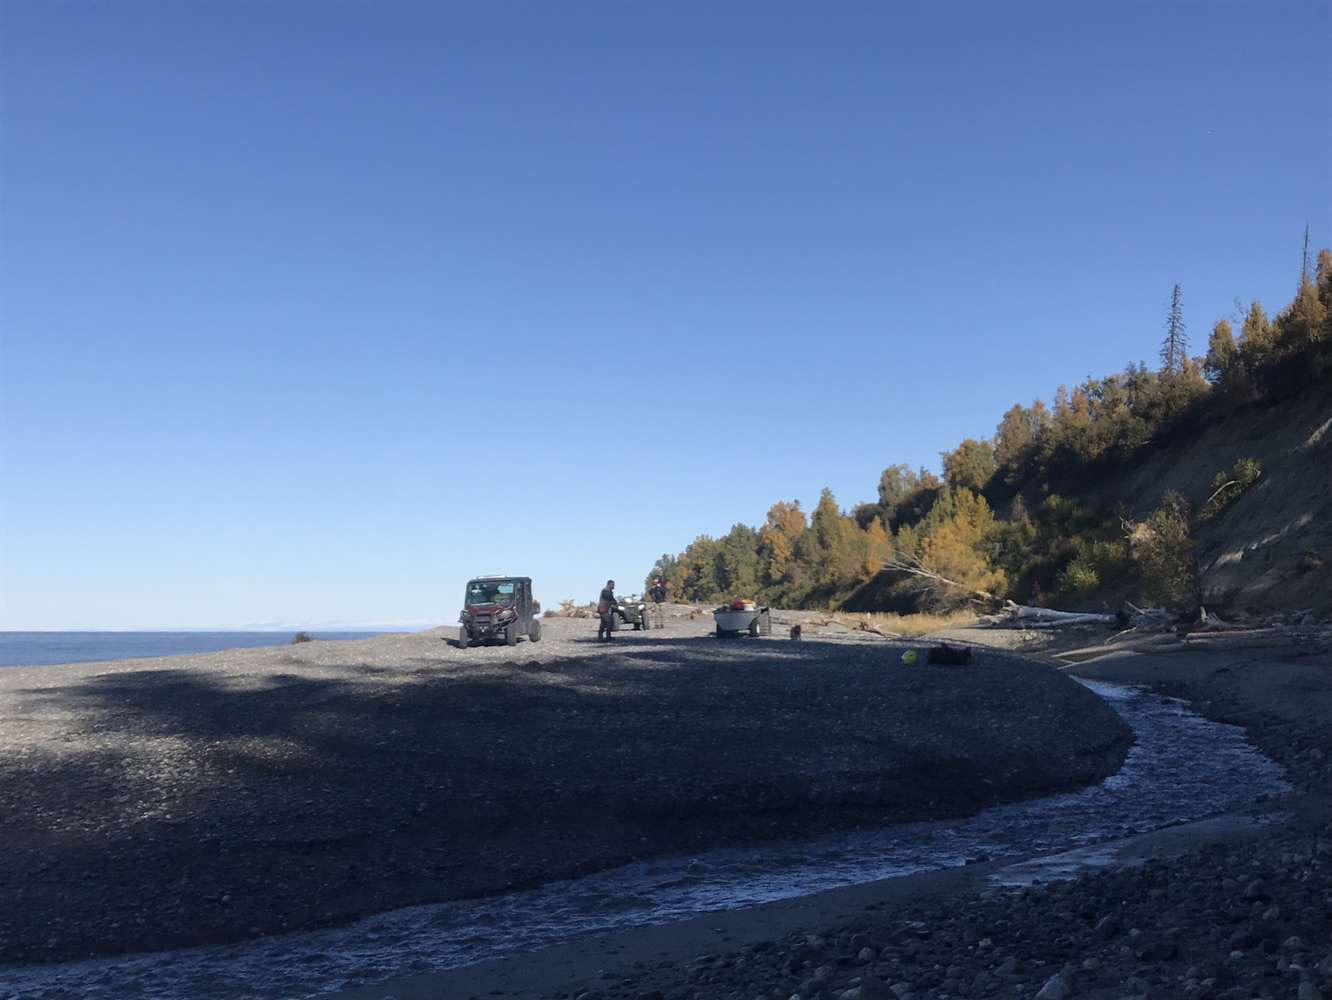
\includegraphics{images/fish_rescue/IMG-0063.jpg}
\caption{\label{fig:unnamed-chunk-19}Mouth of Miller Creek}
\end{figure}

\begin{figure}
\centering
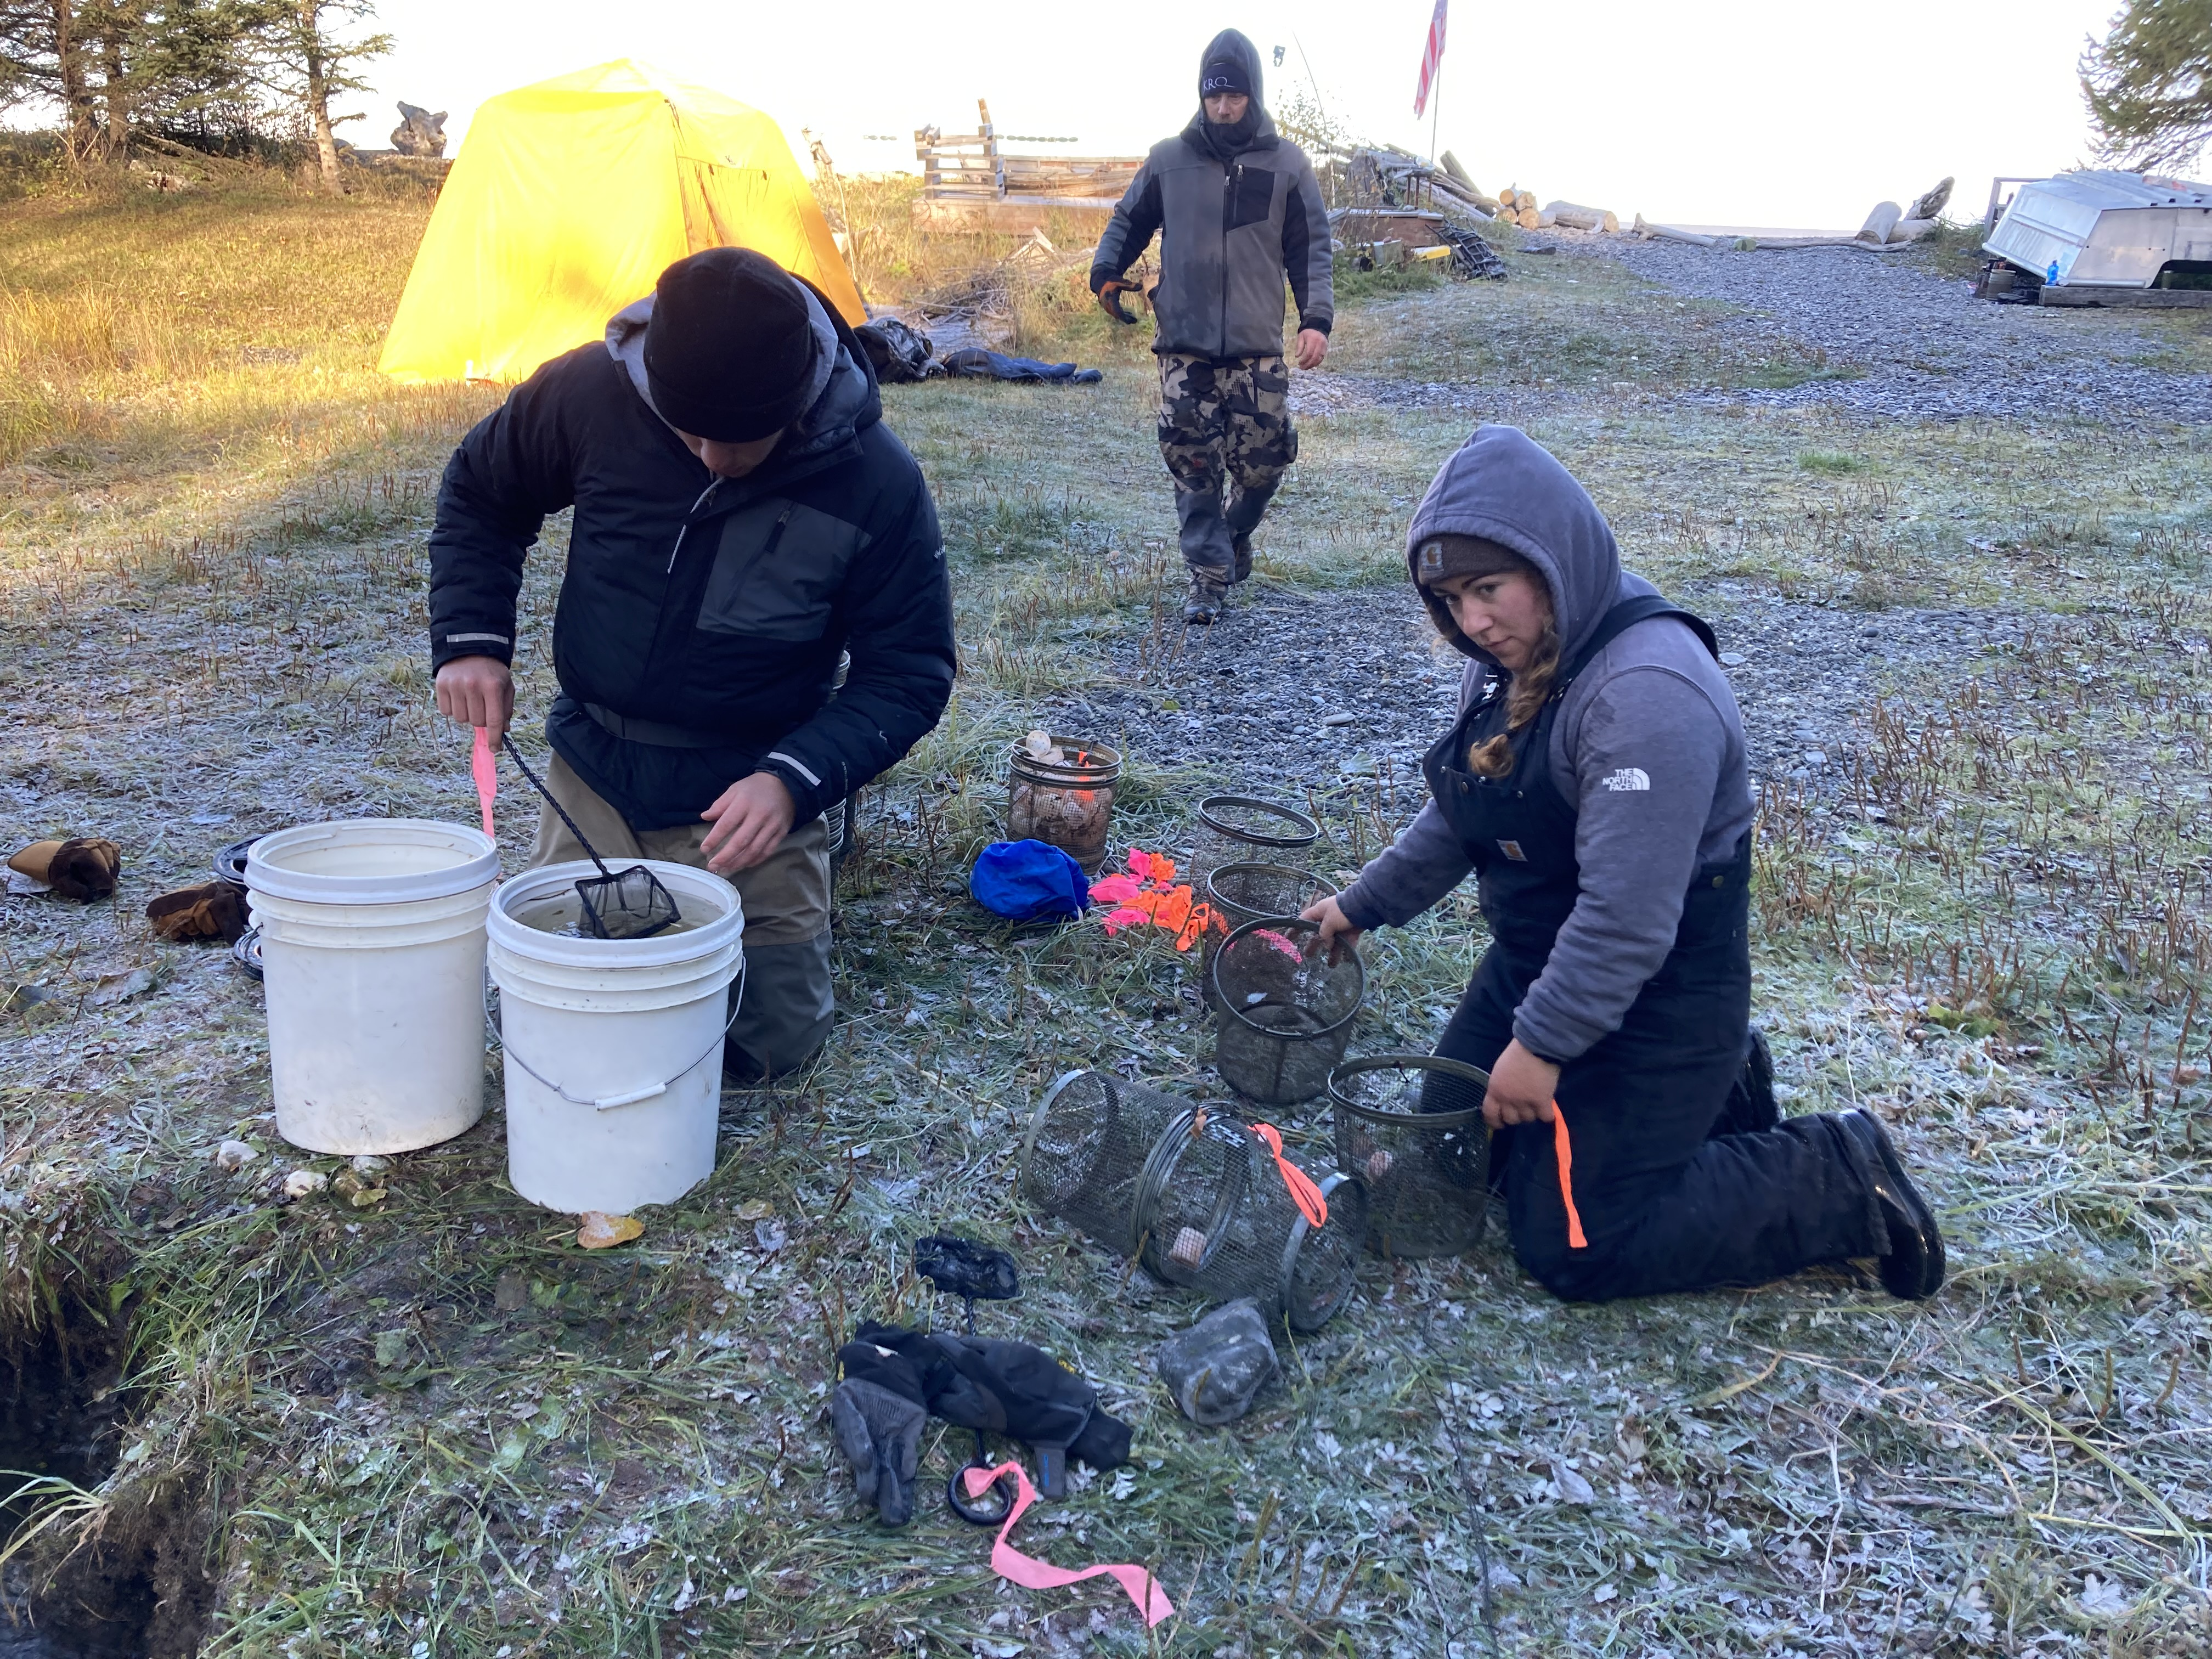
\includegraphics{images/fish_rescue/IMG-6271.jpg}
\caption{\label{fig:unnamed-chunk-20}Fish processing site}
\end{figure}

\begin{figure}
\centering
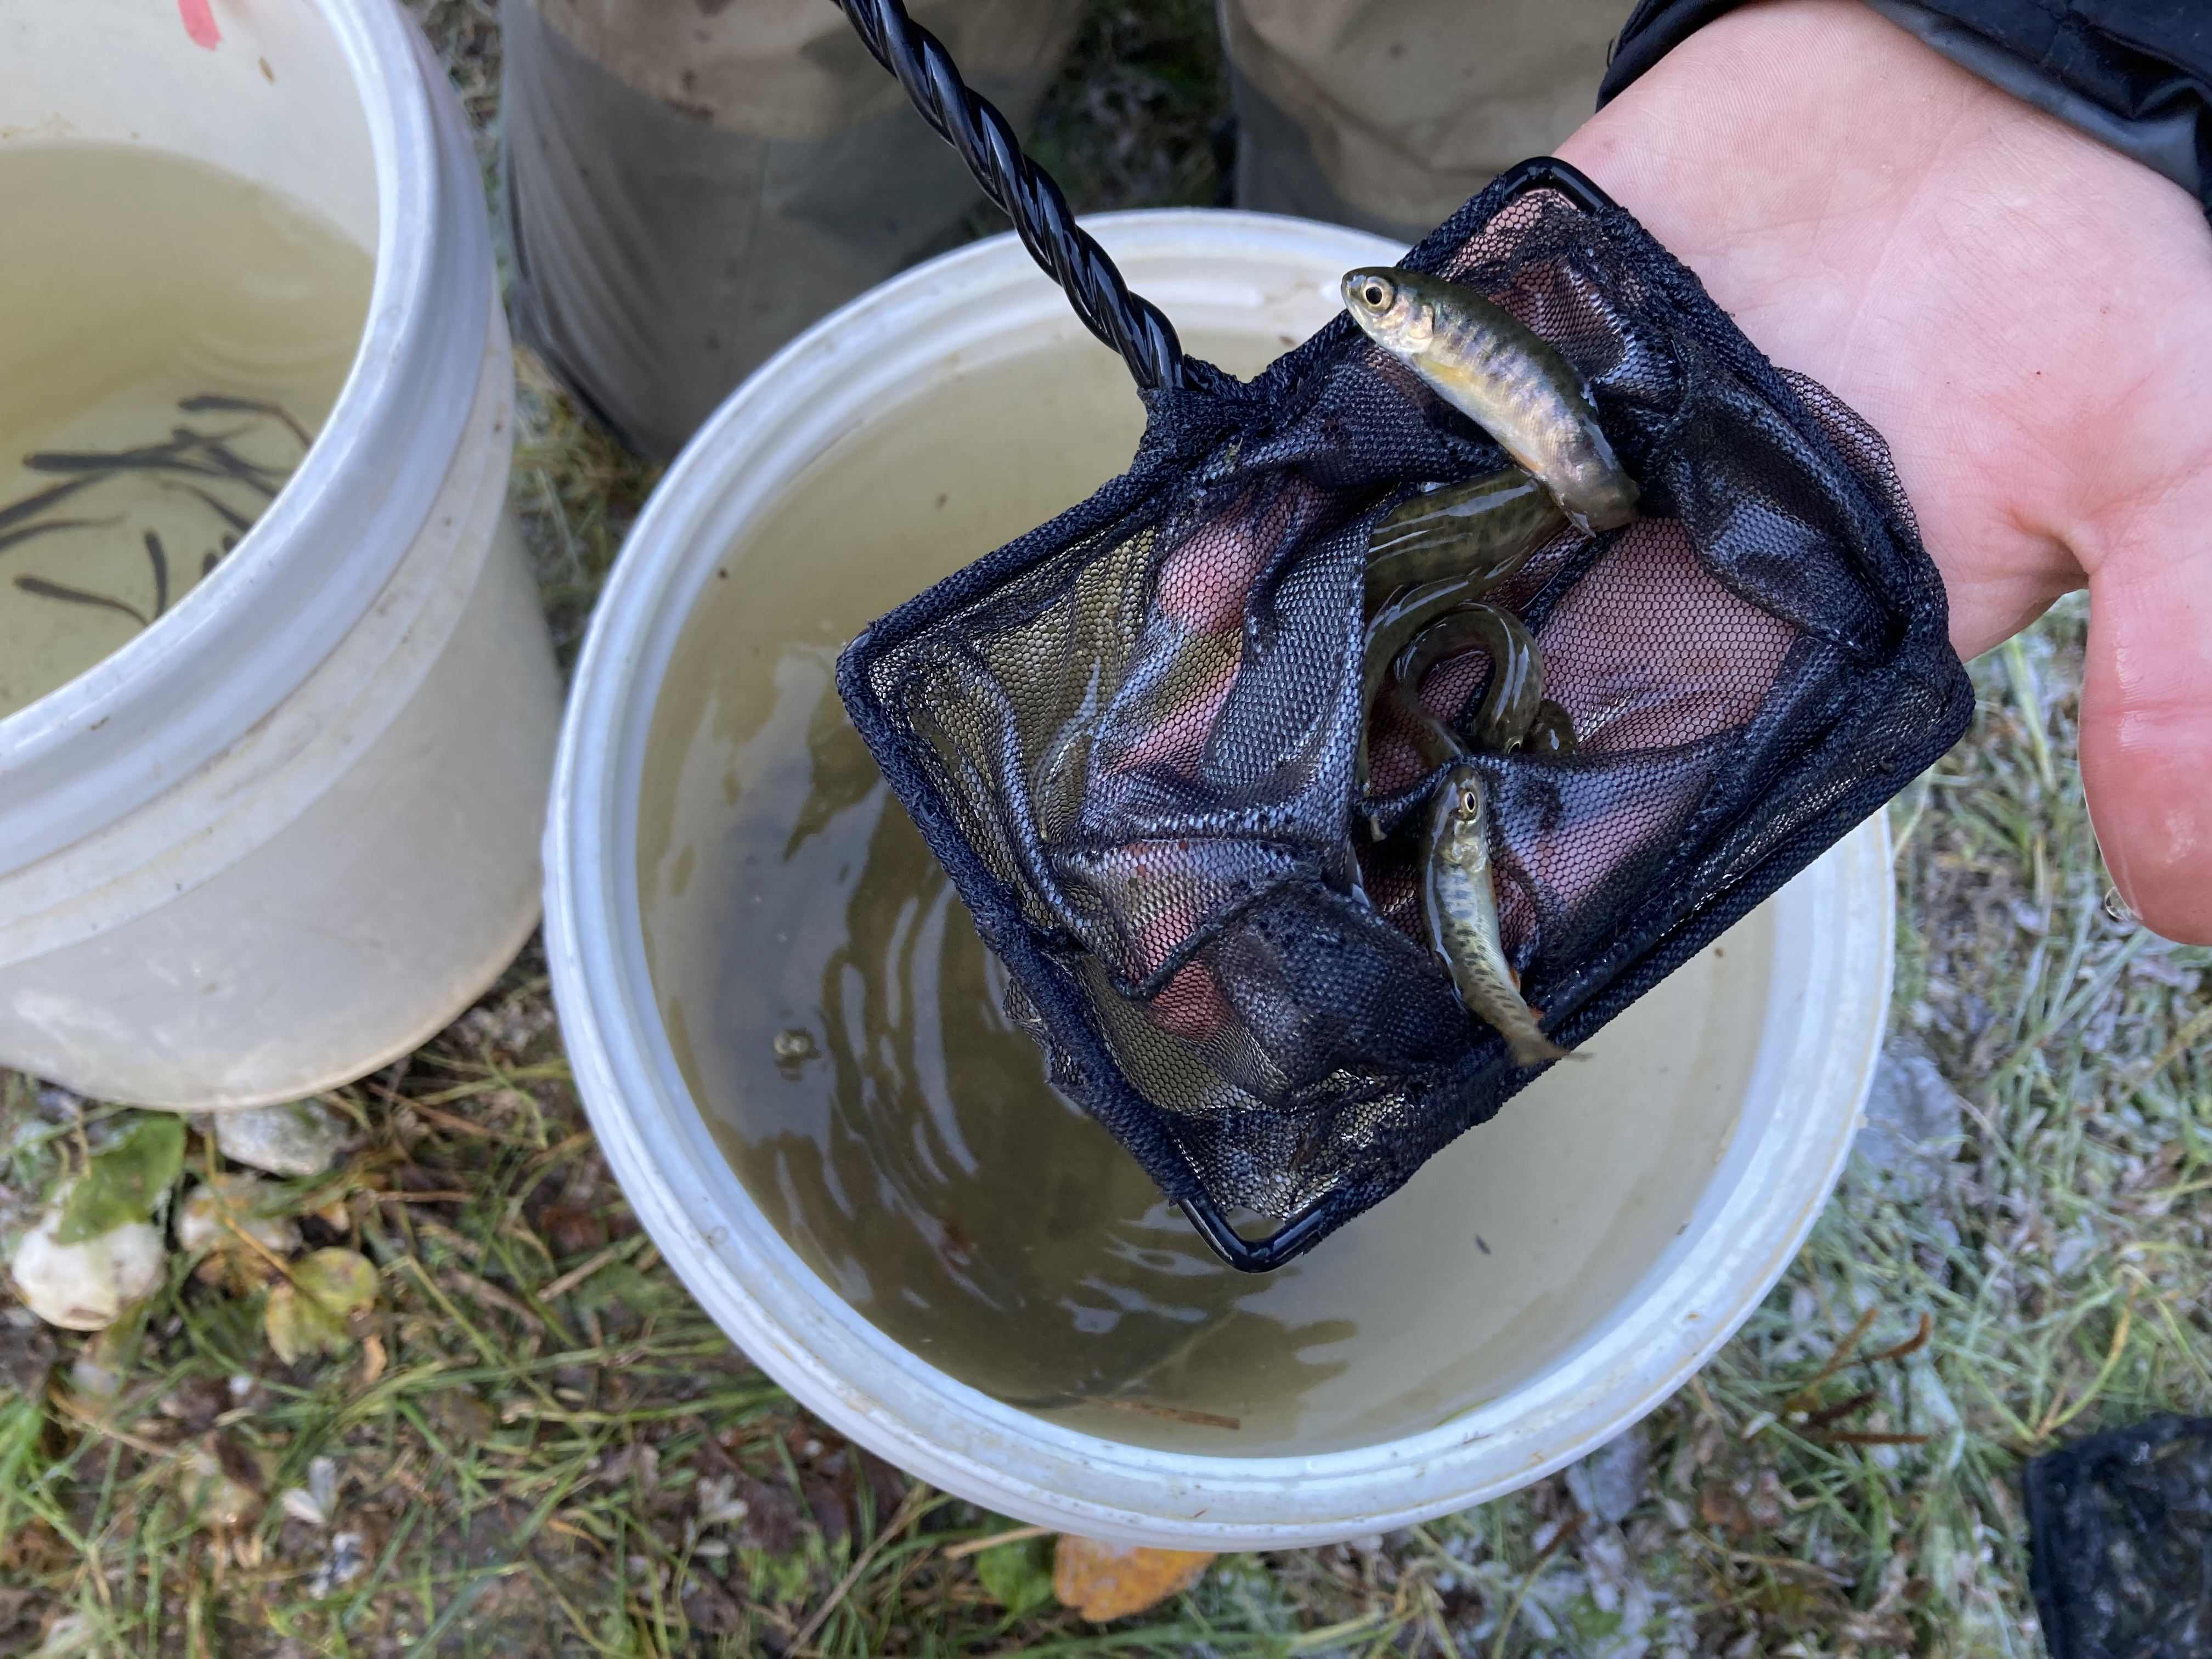
\includegraphics{images/fish_rescue/IMG-6272.jpg}
\caption{\label{fig:unnamed-chunk-21}Juvenile Coho Salmon}
\end{figure}

\begin{figure}
\centering
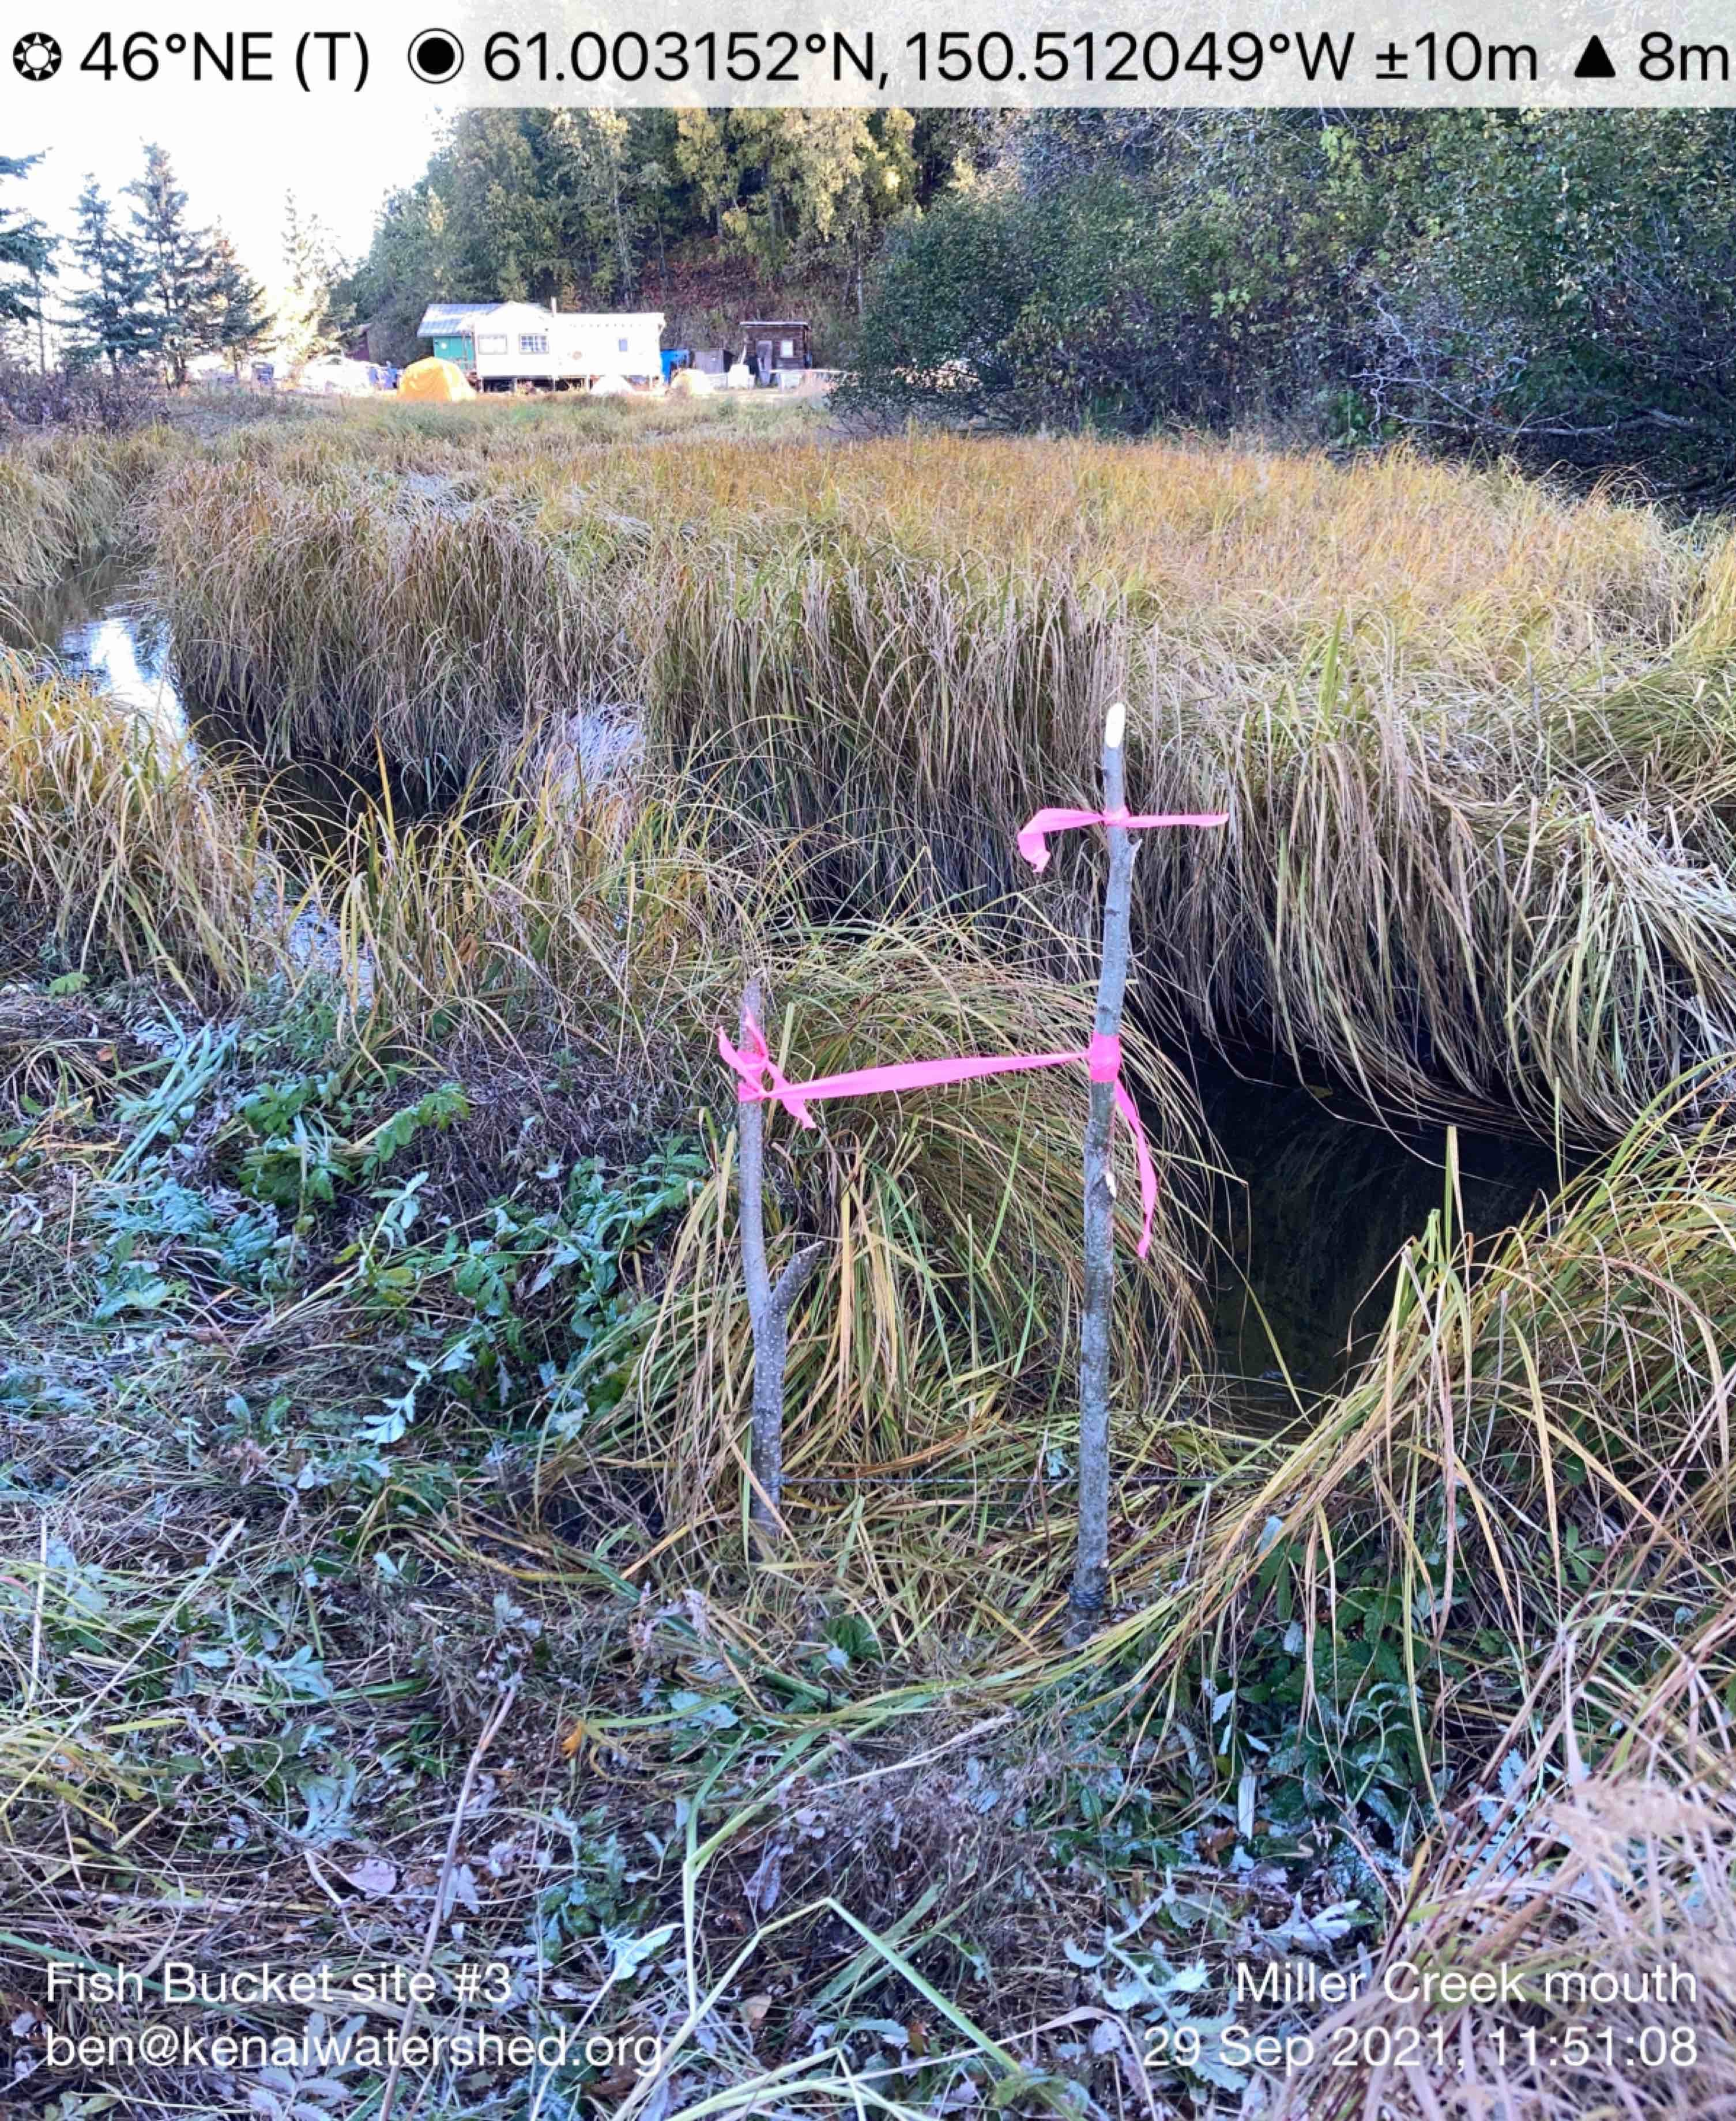
\includegraphics{images/fish_rescue/IMG-6274.jpg}
\caption{\label{fig:unnamed-chunk-22}Site for storage of perforated five-gallon bucket to store juvenile fish}
\end{figure}

\hypertarget{rotenone-monitoring}{%
\chapter{Rotenone monitoring}\label{rotenone-monitoring}}

Rotenone application was performed in early October 2021 by ADF\&G. ADF\&G collected pre and post-treatment water samples as part of this event, and Kenai Watershed Forum will monitor degradation through until Summer 2022. Methods and results will be described here.

\hypertarget{sampling-schedule}{%
\section{Sampling schedule}\label{sampling-schedule}}

A proposed rotenone sampling schedule is described in table \ref{tab:sample-schedule} or may be accessed in a Google Sheet linked here: \url{https://tinyurl.com/8ba94nrn}. Schedule is current as of 2022-01-14.

\begin{table}

\caption{\label{tab:sample-schedule}Vogel lake and Miller Creek rotenone sampling schedule}
\centering
\begin{tabular}[t]{r|l|l|l|l|l|l}
\hline
Field Sample Count & Sample & Field Sample Date & Status & Location & Depth & Notes\\
\hline
1 & Rotenone & 2021-09-27 & Complete & Vogel Lake & Surface & Pre-treatment\\
\hline
1 & Rotenone & 2021-09-28 & Complete & North Vogel Lake & Surface & Pre-treatment\\
\hline
1 & Rotenone & 2021-10-07 & Complete & Vogel Lake & Surface & \\
\hline
1 & Rotenone & 2021-10-07 & Complete & Vogel Lake & Benthic & \\
\hline
1 & Rotenone & 2021-10-07 & Complete & North Vogel Lake & Surface & \\
\hline
1 & Rotenone & 2021-10-07 & Complete & North Vogel Lake & Benthic & \\
\hline
1 & Rotenone & 2021-10-08 & Complete & Miller Creek Head & Surface & \\
\hline
1 & Rotenone & 2021-11-10 & Complete & Miller Creek Weir & Surface & \\
\hline
1 & Rotenone & 2021-11-10 & Complete & North Vogel Lake & Surface & Alternative sampling location due to thin ice\\
\hline
1 & Rotenone & 2021-11-10 & Complete & Vogel Lake & Surface & Alternative sampling location due to thin ice\\
\hline
1 & Rotenone & 2021-12-03 & Complete & Miller Creek & Surface & \\
\hline
1 & Rotenone & 2021-12-02 & Complete & North Vogel Lake & Surface & \\
\hline
1 & Rotenone & 2021-12-02 & Complete & Vogel Lake & Surface & \\
\hline
1 & Rotenone & 2021-12-03 & Complete & Miller Creek & Benthic & \\
\hline
1 & Rotenone & 2021-12-02 & Complete & North Vogel Lake & Benthic & \\
\hline
1 & Rotenone & 2021-12-02 & Complete & Vogel Lake & Benthic & \\
\hline
1 & Rotenone & 2022-01-05 & Complete & Miller Creek & Surface & \\
\hline
1 & Rotenone & 2022-01-05 & Complete & North Vogel Lake & Surface & \\
\hline
1 & Rotenone & 2022-01-05 & Complete & Vogel Lake & Surface & \\
\hline
1 & Rotenone & 2022-03-05 &  & Miller Creek & Surface & \\
\hline
1 & Rotenone & 2022-03-05 &  & North Vogel Lake & Benthic & \\
\hline
1 & Rotenone & 2022-03-05 &  & North Vogel Lake & Surface & \\
\hline
1 & Rotenone & 2022-03-05 &  & Vogel Lake & Benthic & \\
\hline
1 & Rotenone & 2022-03-05 &  & Vogel Lake & Surface & \\
\hline
1 & Rotenone & 2022-05-01 &  & Miller Creek & Surface & \\
\hline
1 & Rotenone & 2022-05-01 &  & North Vogel Lake & Benthic & \\
\hline
1 & Rotenone & 2022-05-01 &  & North Vogel Lake & Surface & \\
\hline
1 & Rotenone & 2022-05-01 &  & Vogel Lake & Benthic & \\
\hline
1 & Rotenone & 2022-05-01 &  & Vogel Lake & Surface & \\
\hline
1 & Rotenone & 2022-06-01 &  & Miller Creek & Surface & \\
\hline
1 & Rotenone & 2022-06-01 &  & North Vogel Lake & Benthic & \\
\hline
1 & Rotenone & 2022-06-01 &  & North Vogel Lake & Surface & \\
\hline
1 & Rotenone & 2022-06-01 &  & Vogel Lake & Benthic & \\
\hline
1 & Rotenone & 2022-06-01 &  & Vogel Lake & Surface & \\
\hline
1 & Rotenone &  &  & TBD & TBD & Date TBD\\
\hline
1 & Rotenone &  &  & TBD & TBD & Date TBD\\
\hline
\end{tabular}
\end{table}

\hypertarget{rotenone-concentration-results}{%
\section{Rotenone concentration results}\label{rotenone-concentration-results}}

\hypertarget{sample-results}{%
\subsection{Sample results}\label{sample-results}}

Laboratory analysis of water samples is performed by the \href{https://www.uaa.alaska.edu/academics/college-of-arts-and-sciences/departments/chemistry/aset_lab/}{ASET Laboratory} at the University of Alaska Anchorage Department of Chemistry in Anchorage, Alaska. Original results to date are available for download at the following link:

\href{https://github.com/Kenai-Watershed-Forum/Miller_Creek_Vogel_Lake_WQX/tree/main/input/rotenone_data}{Link: Rotenone Degradation Laboratory Results}.

Table X\ldots{}

\begin{table}

\caption{(\#tab:results table)Vogel Lake, North Vogel Lake, and Miller Creek rotenone raw results}
\centering
\begin{tabular}[t]{l|l|l|l|r|r|r|l|l|l|l|l}
\hline
sample\_name & lab\_dup & field\_sample\_date & lab\_analysis\_date & rotenone\_ppb & rotenolone\_ppb & deguelin\_ppb & tephrosin\_ppb & cft\_5 & cft\_6 & strata & waterbody\\
\hline
Vogel\_Surface & a & 2021-09-27 & 2021-10-06 & 0.00 & 0.00 & 0.00 & ND & ND & ND & Surface & Vogel\_Lake\\
\hline
Vogel\_Surface & b & 2021-09-27 & 2021-10-06 & 0.00 & 0.00 & 0.00 & ND & ND & ND & Surface & Vogel\_Lake\\
\hline
N\_Vogel\_Surface & a & 2021-09-28 & 2021-10-06 & 0.00 & 0.00 & 0.00 & ND & ND & ND & Surface & N\_Vogel\_Lake\\
\hline
N\_Vogel\_Surface & b & 2021-09-28 & 2021-10-06 & 0.00 & 0.00 & 0.00 & ND & ND & ND & Surface & N\_Vogel\_Lake\\
\hline
Vogel\_Surface & a & 2021-10-07 & 2021-10-13 & 28.26 & 10.59 & 19.94 & Detected & Detected & Detected & Surface & Vogel\_Lake\\
\hline
Vogel\_Surface & b & 2021-10-07 & 2021-10-13 & 22.45 & 10.20 & 19.91 & Detected & Detected & Detected & Surface & Vogel\_Lake\\
\hline
Vogel\_Benthic & a & 2021-10-07 & 2021-10-13 & 18.75 & 9.05 & 16.07 & Detected & Detected & Detected & Benthic & Vogel\_Lake\\
\hline
Vogel\_Benthic & b & 2021-10-07 & 2021-10-13 & 18.36 & 8.60 & 16.02 & Detected & Detected & Detected & Benthic & Vogel\_Lake\\
\hline
N\_Vogel\_Surface & a & 2021-10-07 & 2021-10-13 & 26.97 & 14.30 & 21.57 & Detected & Detected & Detected & Surface & N\_Vogel\_Lake\\
\hline
N\_Vogel\_Surface & b & 2021-10-07 & 2021-10-13 & 26.83 & 14.95 & 21.70 & Detected & Detected & Detected & Surface & N\_Vogel\_Lake\\
\hline
N\_Vogel\_Benthic & a & 2021-10-07 & 2021-10-13 & 13.67 & 7.33 & 10.89 & Detected & Detected & Detected & Benthic & N\_Vogel\_Lake\\
\hline
N\_Vogel\_Benthic & b & 2021-10-07 & 2021-10-13 & 13.54 & 7.90 & 11.22 & Detected & Detected & Detected & Benthic & N\_Vogel\_Lake\\
\hline
Miller\_Creek\_1 &  & 2021-10-08 & 2021-10-13 & 22.96 & 13.27 & 19.78 & Detected & Detected & Detected & Creek & Miller\_Creek\\
\hline
Vogel\_Surface & a & 2021-11-10 & 2021-11-12 & 12.39 & 7.69 & 9.24 & Detected & Detected & Detected & Surface & Vogel\_Lake\\
\hline
Vogel\_Surface & b & 2021-11-10 & 2021-11-12 & 13.08 & 8.50 & 9.59 & Detected & Detected & Detected & Surface & Vogel\_Lake\\
\hline
N\_Vogel\_Surface & a & 2021-11-10 & 2021-11-12 & 15.05 & 10.87 & 10.27 & Detected & Detected & Detected & Surface & N\_Vogel\_Lake\\
\hline
N\_Vogel\_Surface & b & 2021-11-10 & 2021-11-12 & 15.62 & 11.77 & 10.28 & Detected & Detected & Detected & Surface & N\_Vogel\_Lake\\
\hline
Miller Creek Weir & a & 2021-11-10 & 2021-11-12 & 2.03 & 5.52 & 1.01 & Detected & ND & ND & Creek & Miller\_Creek\\
\hline
Miller Creek Weir & b & 2021-11-10 & 2021-11-12 & 1.99 & 4.99 & 1.06 & Detected & ND & ND & Creek & Miller\_Creek\\
\hline
Vogel\_Surface & a & 2021-12-02 & 2021-12-06 & 8.79 & 7.63 & 6.25 & Detected & Detected & Detected & Surface & Vogel\_Lake\\
\hline
Vogel\_Surface & b & 2021-12-02 & 2021-12-06 & 8.83 & 6.98 & 6.26 & Detected & Detected & Detected & Surface & Vogel\_Lake\\
\hline
Vogel\_Benthic & a & 2021-12-02 & 2021-12-06 & 10.79 & 8.54 & 7.52 & Detected & Detected & Detected & Benthic & Vogel\_Lake\\
\hline
Vogel\_Benthic & b & 2021-12-02 & 2021-12-06 & 10.64 & 8.54 & 7.39 & Detected & Detected & Detected & Benthic & Vogel\_Lake\\
\hline
N\_Vogel\_Surface & a & 2021-12-02 & 2021-12-06 & 13.81 & 12.26 & 8.57 & Detected & Detected & Detected & Surface & N\_Vogel\_Lake\\
\hline
N\_Vogel\_Surface & b & 2021-12-02 & 2021-12-06 & 13.61 & 11.64 & 8.56 & Detected & Detected & Detected & Surface & N\_Vogel\_Lake\\
\hline
N\_Vogel\_Benthic & a & 2021-12-02 & 2021-12-06 & 11.78 & 10.85 & 7.59 & Detected & Detected & Detected & Benthic & N\_Vogel\_Lake\\
\hline
N\_Vogel\_Benthic & b & 2021-12-02 & 2021-12-06 & 12.78 & 12.58 & 7.96 & Detected & Detected & Detected & Benthic & N\_Vogel\_Lake\\
\hline
Miller\_Creek\_2 & a & 2021-12-03 & 2021-12-06 & 6.32 & 6.83 & 4.59 & Detected & Detected & Detected & Creek & Miller\_Creek\\
\hline
Miller\_Creek\_2 & b & 2021-12-03 & 2021-12-06 & 6.85 & 6.93 & 4.77 & Detected & Detected & Detected & Creek & Miller\_Creek\\
\hline
\end{tabular}
\end{table}

\begin{Shaded}
\begin{Highlighting}[]
\DocumentationTok{\#\# lakes plot}

\FunctionTok{ggplotly}\NormalTok{(rot\_dat }\SpecialCharTok{\%\textgreater{}\%}
    \CommentTok{\# remove miller creek}
      \FunctionTok{filter}\NormalTok{(waterbody }\SpecialCharTok{!=} \StringTok{"Miller\_Creek"}\NormalTok{) }\SpecialCharTok{\%\textgreater{}\%}
    \FunctionTok{group\_by}\NormalTok{(sample\_name,field\_sample\_date, waterbody,strata) }\SpecialCharTok{\%\textgreater{}\%}
    \FunctionTok{summarise}\NormalTok{(}\AttributeTok{avg\_rotenone\_ppb =} \FunctionTok{mean}\NormalTok{(rotenone\_ppb)) }\SpecialCharTok{\%\textgreater{}\%}
  
    \FunctionTok{ggplot}\NormalTok{(}\FunctionTok{aes}\NormalTok{(field\_sample\_date,avg\_rotenone\_ppb, }\AttributeTok{color =}\NormalTok{ strata)) }\SpecialCharTok{+}
    \FunctionTok{geom\_point}\NormalTok{() }\SpecialCharTok{+}
    \FunctionTok{geom\_line}\NormalTok{() }\SpecialCharTok{+}
    \FunctionTok{facet\_grid}\NormalTok{(. }\SpecialCharTok{\textasciitilde{}}\NormalTok{ waterbody) }\SpecialCharTok{+}
      \FunctionTok{xlab}\NormalTok{(}\StringTok{""}\NormalTok{) }\SpecialCharTok{+}
      \FunctionTok{ylab}\NormalTok{(}\StringTok{"Rotenone Concentration (ppb)"}\NormalTok{)}
\NormalTok{  )}
  

\CommentTok{\# say that more detailed accuracy results can be accessed in the repo folder in the excel files}

\CommentTok{\# see journal article for methods}
\end{Highlighting}
\end{Shaded}

\begin{Shaded}
\begin{Highlighting}[]
\DocumentationTok{\#\# creek plot}

\DocumentationTok{\#\# join data with location estimates (distance down creek)}


\FunctionTok{ggplotly}\NormalTok{(rot\_dat }\SpecialCharTok{\%\textgreater{}\%}
    \CommentTok{\# include miller creek}
      \FunctionTok{filter}\NormalTok{(waterbody }\SpecialCharTok{==} \StringTok{"Miller\_Creek"}\NormalTok{) }\SpecialCharTok{\%\textgreater{}\%}
    \FunctionTok{group\_by}\NormalTok{(sample\_name,field\_sample\_date, waterbody,strata) }\SpecialCharTok{\%\textgreater{}\%}
    \FunctionTok{summarise}\NormalTok{(}\AttributeTok{avg\_rotenone\_ppb =} \FunctionTok{mean}\NormalTok{(rotenone\_ppb)) }\SpecialCharTok{\%\textgreater{}\%}
  
    \FunctionTok{ggplot}\NormalTok{(}\FunctionTok{aes}\NormalTok{(field\_sample\_date,avg\_rotenone\_ppb, }\AttributeTok{color =}\NormalTok{ strata)) }\SpecialCharTok{+}
    \FunctionTok{geom\_point}\NormalTok{() }\SpecialCharTok{+}
    \FunctionTok{geom\_line}\NormalTok{() }\SpecialCharTok{+}
    \FunctionTok{facet\_grid}\NormalTok{(. }\SpecialCharTok{\textasciitilde{}}\NormalTok{ waterbody) }\SpecialCharTok{+}
      \FunctionTok{xlab}\NormalTok{(}\StringTok{""}\NormalTok{) }\SpecialCharTok{+}
      \FunctionTok{ylab}\NormalTok{(}\StringTok{"Rotenone Concentration (ppb)"}\NormalTok{)}
\NormalTok{  )}
\end{Highlighting}
\end{Shaded}

\hypertarget{summary-1}{%
\chapter{Summary}\label{summary-1}}

Overall results described and interpreted here.

  \bibliography{book.bib,packages.bib}

\end{document}
